\chapter{退相干与多电子关联}

前几章主要从闭合电子--光场系统的幺正演化出发。实验并不会同时记录材料中的每个电子--空穴激发、每个声子以及每一次相位漂移。那些没有被测量的自由度会带走哪一路信息，于是电子密度矩阵的非对角元开始衰减。

退相干模型应尽可能追溯到环境相关函数、材料损耗谱或技术噪声，而不应仅用一个未说明来源的常数 $\gamma$ 取代所有机制。在此基础上，整形电子驱动三能级系统的鲁棒性问题可表述为：当相位、失谐和耗散参数存在偏差时，目标路径干涉能否保持。

系统、环境分别记为 $S,E$，总耦合强度以 $\lambda$ 计阶。耗散子采用 $\mathcal D[L]\rho=L\rho L^\dagger-\tfrac12\{L^\dagger L,\rho\}$。Born、Markov 与久期近似是彼此不同的近似步骤：分别限制系统--环境关联、环境记忆时间和不同 Bohr 频率项的相互平均；若这些时间尺度不分离，GKSL 半群方程不应被无条件使用。


\section{开放系统动力学}
只看电子时，电子态一般不会保持纯态。原因不是总体系违反幺正演化，而是实验没有同时读取环境。设电子为系统 $S$，未观测的光子、声子或材料激发为环境 $E$。总哈密顿量写成

\begin{equation}
H_{SE}=H_S+H_E+\lambda\sum_\alpha A_\alpha\otimes B_\alpha,
\label{eq:ch05-1}
\end{equation}

$A_\alpha$ 作用在电子 Hilbert 空间，$B_\alpha$ 作用在环境 Hilbert 空间，$\lambda$ 表示系统—环境耦合强度。总密度算符满足精确的 von Neumann 方程。进入相互作用绘景后，只有相互作用项保留下来：

\begin{equation}
\frac{\dd \widetilde\rho_{SE}}{\dd t}=-\frac{\ii\lambda}{\hbar}[\widetilde H_I(t),\widetilde\rho_{SE}(t)].
\label{eq:ch05-2}
\end{equation}

为从这个精确的总态演化得到电子动力学，应先把\cref{eq:ch05-2} 积分一次，然后将积分形式代回右侧。令 $\widetilde H_I(t)=\sum_\alpha\widetilde A_\alpha(t)\otimes\widetilde B_\alpha(t)$（不含显式因子 $\lambda$），得到
\begin{align*}
\widetilde\rho_{SE}(t)
&=\widetilde\rho_{SE}(0)
-\frac{\ii\lambda}{\hbar}\int_0^t\dd s\,
[\widetilde H_I(s),\widetilde\rho_{SE}(s)],\\
\frac{\dd\widetilde\rho_S(t)}{\dd t}
&=-\frac{\ii\lambda}{\hbar}\operatorname{Tr}_E
[\widetilde H_I(t),\widetilde\rho_{SE}(0)]\\
&\quad-\frac{\lambda^2}{\hbar^2}\int_0^t\dd s\,
\operatorname{Tr}_E[\widetilde H_I(t),
[\widetilde H_I(s),\widetilde\rho_{SE}(s)]].
\end{align*}
这仍是严格恒等式：右边依赖未知的联合态 $\widetilde\rho_{SE}(s)$，没有把它偷换成电子单独的密度算符。现在明确指定初始无关联条件
$\widetilde\rho_{SE}(0)=\rho_S(0)\otimes\rho_E$，其中
$[H_E,\rho_E]=0$，并选择中心化的环境算符
$\operatorname{Tr}_E(B_\alpha\rho_E)=0$。若环境算符原来不满足最后一式，可把其均值对应的一阶哈密顿量吸收到 $H_S$。在这些条件下，上式中的一阶项严格消失，留下

\begin{equation}
\dot{\widetilde\rho}_S(t)=-\frac{\lambda^2}{\hbar^2}\int_0^t \dd s\;\operatorname{Tr}_E\!\left[\widetilde H_I(t),[\widetilde H_I(s),\widetilde\rho_{SE}(s)]\right],
\label{eq:ch05-3}
\end{equation}

由于\cref{eq:ch05-3} 仍含未知的 $\widetilde\rho_{SE}(s)$，它并没有构成可直接求解的电子封闭方程。弱耦合处理的第一步是玻恩近似：在保留到 $O(\lambda^2)$ 的精度下，取 $\widetilde\rho_{SE}(s)\simeq\widetilde\rho_S(s)\otimes\rho_E$。它忽略的是系统与环境在积分核中积累的高阶关联。

若环境关联函数在时间 $\tau_E$ 内衰减，而电子态只在更长的 $\tau_S$ 上明显变化，即 $\tau_E\ll\tau_S$，则积分主要来自 $s\approx t$。这时可以把 $\widetilde\rho_S(s)$ 换成 $\widetilde\rho_S(t)$，并把积分上限延到无穷大。这一步是马尔可夫近似；它丢掉了环境的长时间记忆。

最后把系统算符按 $H_S$ 的 Bohr 频率分解为 $A_\alpha(\omega)$。若不同 Bohr 频率之间的拍频远快于耗散时间，即 $|\omega-\omega'|\tau_S\gg1$，时间平均会压低 $\omega\ne\omega'$ 的交叉项。做这一旋转波（久期）近似后，生成元可写成 Gorini--Kossakowski--Sudarshan--Lindblad（GKSL）形式：

\begin{equation}
\dot\rho_S=-\frac{i}{\hbar}[H_S+H_{\mathrm{LS}},\rho_S]+\sum_{\omega,\alpha,\beta}\gamma_{\alpha\beta}(\omega)\left[A_\beta(\omega)\rho_S A_\alpha^\dagger(\omega)-\frac12\{A_\alpha^\dagger(\omega)A_\beta(\omega),\rho_S\}\right].
\label{eq:ch05-4}
\end{equation}

$H_{\mathrm{LS}}$ 是环境引起的 Lamb 位移。速率矩阵由环境关联函数的傅里叶变换给出：

\begin{equation*}
\gamma_{\alpha\beta}(\omega)=\frac{\lambda^2}{\hbar^2}\int_{-\infty}^{\infty}\dd \tau\,\ee^{\ii\omega\tau}\langle B_\alpha(\tau)B_\beta(0)\rangle_E.
\end{equation*}

环境相关谱为什么能够给出非负的 GKSL 速率，而不只是形式上的 Fourier 变换？这里选择厄米的环境耦合算符 $B_\alpha$；一般非厄米耦合可拆成厄米与反厄米部分，并相应扩充算符指标。对任意复系数 $z_\alpha$，定义环境算符 $C(t)=\sum_\alpha z_\alpha B_\alpha(t)$。在平稳环境中，以 $X_T=\int_0^T\dd t\,\ee^{-\ii\omega t}C(t)$ 构造有限时间的算符积分，就有
\begin{align*}
\sum_{\alpha\beta}z_\alpha^*\gamma_{\alpha\beta}(\omega)z_\beta
&=\frac{\lambda^2}{\hbar^2}\lim_{T\to\infty}\frac1T
\langle X_T^\dagger X_T\rangle_E\ge0.
\end{align*}
极限用到了环境相关函数随时间差足够快衰减，从而将双重时间积分的三角窗延展成全频 Fourier 积分。因为 $X_T^\dagger X_T$ 是正算符，所有复向量 $\vb z$ 的二次型都非负，所以 $\gamma(\omega)$ 是半正定矩阵。它可以对角化成非负本征值与对应跳跃算符，正是 GKSL 耗散子保持完全正性的数学条件；若任意指定一组负的“衰减率”，一般就得不到这样的微观推导。

这里将总相互作用写为 $\lambda\sum_\alpha A_\alpha\otimes B_\alpha$，所以速率中必须包含 $\lambda^2$；若把耦合强度预先吸收入 $B_\alpha$，才可省略这个显式因子。退相干率由环境在相应 Bohr 频率处的关联谱以及系统耦合算符共同决定。

这条推导链同时给出适用条件：耦合不能强到玻恩近似的二阶截断失效，环境记忆不能与系统时间尺度相当，且近简并跃迁不能被久期近似错误地分开。任一条件不满足时，\cref{eq:ch05-4} 仍可作为模型使用，但不能再把它称为从微观哈密顿量受控推出的 Markov 主方程。

\textsuperscript{\hyperref[ch05-ref4]{[4]}}
GKSL 方程告诉我们怎样保证约化动力学保持完全正性，却不会自动告诉我们某块真实材料的退相干率是多少。对电子显微中的空间相干，更直接的对象是电子实空间密度矩阵。Velasco、Di Giulio 与 García de Abajo 在 2026 年把自由电子与材料和电磁环境的耦合写成统一的密度矩阵传播；在无反冲近似下，作用后的电子态可以写成
\begin{equation}
\rho_f(\vb r,\vb r')
=e^{-P(\vb r,\vb r')+\ii\chi(\vb r,\vb r')}
\rho_i(\vb r,\vb r').
\label{eq:ch05-material-decoherence}
\end{equation}
这里 $\chi$ 是弹性相位，而 $P\ge0$ 描述环境带走哪一路信息后造成的相干衰减。对角元满足 $P(\vb r,\vb r)=0$，因此这个因子不直接删除位置概率；它首先压低的是 $\vb r\neq\vb r'$ 的非对角相干。

这条式子的物理内容可以从两条路径 $A,B$ 看得最清楚。若两条路径激发环境的振幅几乎相同，环境无法判断电子走了哪一路，交叉项会抵消大部分局域损失贡献，$P(A,B)$ 很小；若两条路径激发的模式在空间上高度局域、相位和幅度明显不同，环境获得了路径信息，$P(A,B)$ 增大。干涉可见度因此近似按
\begin{equation}
\mathcal V_f\simeq \mathcal V_i e^{-P(A,B)}
\label{eq:ch05-visibility-material}
\end{equation}
衰减。这里的关键不是“发生一次能量损失就完全退相干”，而是两条路径对环境留下的状态是否可区分。

前面以材料响应核描述两条电子路径的相干衰减，但衰减因子为何必然取环境态的重叠形式，以及相干信息究竟去了哪里，还可以从一个不依赖马尔可夫近似的精确量子模型看出来。设电子有两条可区分的路径 $|A\rangle,|B\rangle$，环境初态是真空 $|0\rangle_\gamma$。电子走不同路径时使同一个光学模式分别产生复位移 $\alpha_A,\alpha_B$，总演化取为
\begin{equation}
U_{SE}=|A\rangle\langle A|\otimes D(\alpha_A)
+|B\rangle\langle B|\otimes D(\alpha_B),
\qquad D(\alpha)=\ee^{\alpha a^\dagger-\alpha^*a}.
\label{eq:env-controlled-displacement}
\end{equation}
两条电子路径上的算符是正交投影，而每一个位移算符自身都是幺正的，因此 $U_{SE}^\dagger U_{SE}=\mathbb I$；这是一种完整的可逆联合演化。对于入射电子 $\sqrt p|A\rangle+\ee^{\ii\phi}\sqrt{1-p}|B\rangle$，作用后得到
\[
|\Psi_{SE}\rangle=\sqrt p|A\rangle|\alpha_A\rangle
+\ee^{\ii\phi}\sqrt{1-p}|B\rangle|\alpha_B\rangle,
\]
其中 $|\alpha\rangle=D(\alpha)|0\rangle$ 是归一化相干态。把环境迹掉以后，电子不再由单个波函数描述；路径基中的非对角矩阵元为
\begin{align*}
\rho_{AB}
&=\sqrt{p(1-p)}\,\ee^{-\ii\phi}\langle\alpha_B|\alpha_A\rangle,\\
\langle\alpha_B|\alpha_A\rangle
&=\exp\!\left[-\frac{|\alpha_A|^2+|\alpha_B|^2}{2}
+\alpha_B^*\alpha_A\right]\\
&=\exp\!\left[-\frac{|\alpha_A-\alpha_B|^2}{2}
+\ii\operatorname{Im}(\alpha_B^*\alpha_A)\right].
\end{align*}
这里第二行是用位移算符的乘法公式
$D^\dagger(\alpha_B)D(\alpha_A)
=\ee^{\ii\operatorname{Im}(\alpha_B^*\alpha_A)}D(\alpha_A-\alpha_B)$
以及 $\langle0|D(\delta)|0\rangle=\ee^{-|\delta|^2/2}$ 得到的。环境不仅压低相干振幅，还可能带来一项可测相位。由此可得与一般材料核同一结构的\emph{精确}相干因子
\begin{equation}
|\rho_{AB}|=\sqrt{p(1-p)}\ee^{-\mathcal P},\qquad
\mathcal P=\frac12|\alpha_A-\alpha_B|^2.
\label{eq:env-overlap-decay}
\end{equation}
两条路径各自可以强烈激发环境，但只要 $\alpha_A=\alpha_B$，环境得到的状态就完全一样，电子便不失去干涉可见度；相反，即使局域平均损失不大，只要两个环境输出态足够可区分，电子干涉也会被洗掉。这里的 $\mathcal P$ 是单次散射后的无量纲相干衰减指数，不应不加时间模型就写成 $\gamma t$。

为了把“环境区分了路径”变成定量可测的命题，取等权入射 $p=1/2$，并选择相位参考使 $\alpha_A=\delta/2$、$\alpha_B=-\delta/2$ 为实数。两环境态的内积模为 $d=\ee^{-\delta^2/2}$，电子在互补路径基中的干涉可见度就是 $\mathcal V=d$。由于联合态仍然是纯态，电子与环境的纠缠熵可以直接由电子的两个本征值 $\lambda_\pm=(1\pm d)/2$ 得出：
\begin{equation}
S(\rho_e)=-\sum_{\nu=\pm}\lambda_\nu\log_2\lambda_\nu,
\qquad \operatorname{Tr}\rho_e^2=\frac{1+d^2}{2}.
\label{eq:env-purity-entropy}
\end{equation}
如果实验允许对环境做最优的两态判别，等先验纯态的 Helstrom 可区分度为 $\mathcal D=\sqrt{1-d^2}$，最小误判概率为 $(1-\mathcal D)/2$。因此
\begin{equation}
\mathcal V^2+\mathcal D^2=1.
\label{eq:env-complementarity}
\end{equation}
这不是把光子数损失等同于退相干，而是把两条环境\emph{输出态}在 Hilbert 空间中的距离与电子条纹对比度直接联系起来。

环境中存在路径信息，也不意味着所有单次后选择实验都必须失去条纹。定义归一化的环境叠加态
$|e_\pm\rangle=(|\delta/2\rangle\pm|-\delta/2\rangle)/\sqrt{2(1\pm d)}$。
在这些正交基上测量后，两个条件电子态分别与
$(|A\rangle\pm\ee^{\ii\phi}|B\rangle)/\sqrt2$ 成正比。它们的成功概率为 $p_\pm=(1\pm d)/2$，条件干涉概率分别为
\[
P_\pm(\varphi)=\frac{1\pm\cos\varphi}{2},\qquad
P_{\rm uncond}(\varphi)=\sum_{\nu=\pm}p_\nu P_\nu(\varphi)
=\frac{1+d\cos\varphi}{2}.
\]
条件条纹重新达到单位可见度，是因为环境测量选择了擦去路径标签的叠加基；两组条纹相位相反，把记录丢掉后又恢复到原来的低对比度。这种“量子擦除”依赖可访问且可相干测量的环境模式。对无法收集的材料电子--空穴激发，不能简单将这个理想操作当成可用的实验反馈。

\begin{figure}[!htbp]
\centering
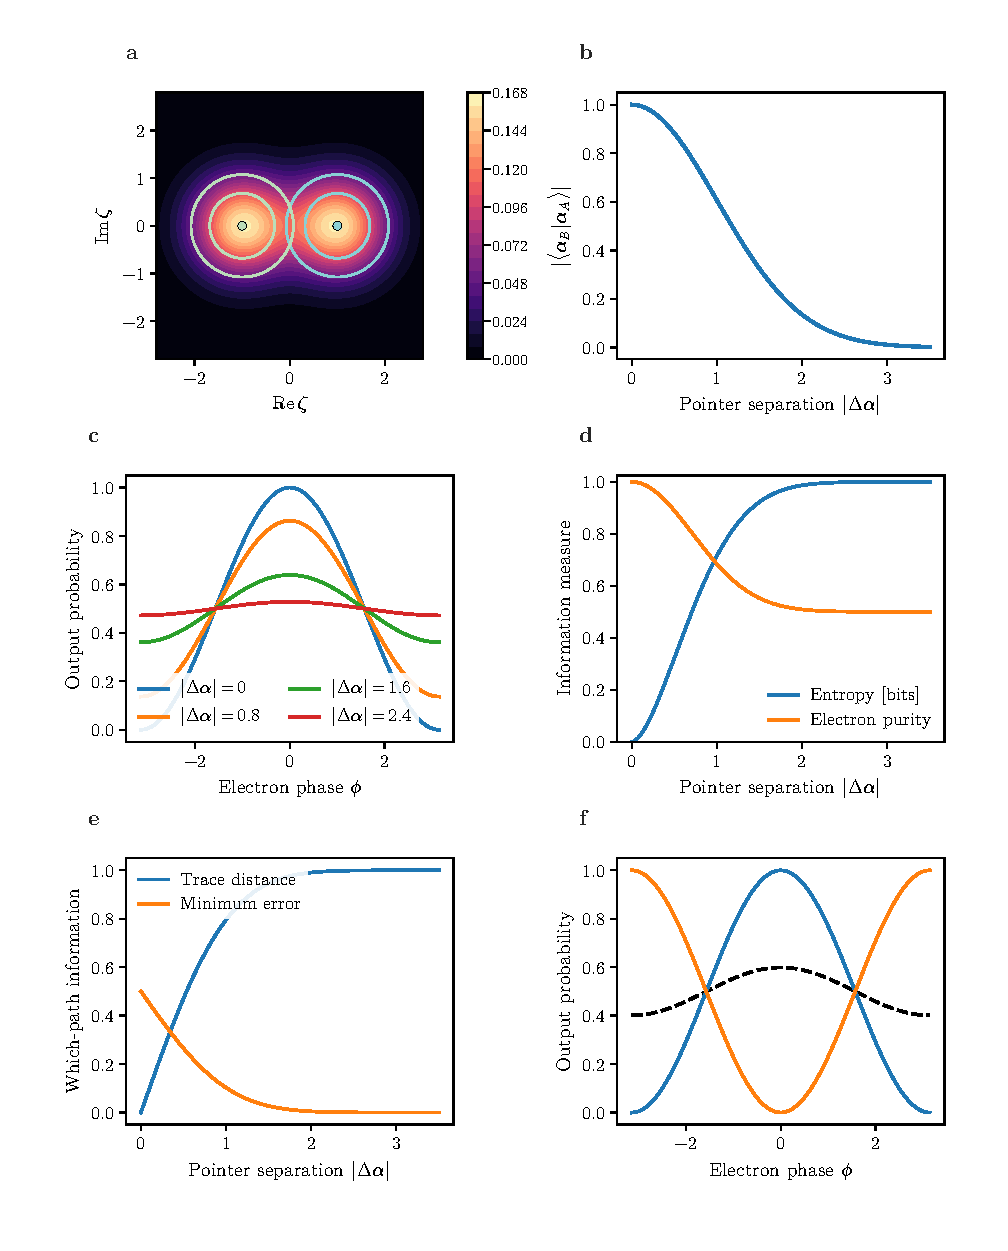
\includegraphics[width=0.96\linewidth,height=0.70\textheight,keepaspectratio]{environment_pointer_eraser.pdf}
\caption{\textbf{从环境态重叠到退相干、路径辨别与量子擦除。} 全图使用精确条件位移模型\cref{eq:env-controlled-displacement}。(a) 取 $\delta=2$，绘两条电子路径对应光学相干态的 Husimi $Q$ 分布及其等权混合，展示环境指针在相空间中的分离。(b) 环境态重叠 $d=\ee^{-\delta^2/2}$ 随指针距离的下降。(c) $\delta=0,0.8,1.6,2.4$ 的无条件电子干涉条纹。(d) 电子纯度与电子--环境纠缠熵，这两个量均由同一个 $d$ 精确给出。(e) 最优环境路径判别的迹距离和 Helstrom 最小误判概率。(f) 固定 $\delta=1.8$，黑色虚线是无条件干涉；蓝色和橙色实线是环境擦除测量两个互补结果的条件干涉，它们具有相反条纹相位。所示结果不是特定材料的耗散拟合。}
\label{fig:environment-pointer-eraser}
\end{figure}

定义条件环境态为 $|\alpha_A\rangle=|\delta/2\rangle$、$|\alpha_B\rangle=|-\delta/2\rangle$，两条路径初始权重都为 $1/2$，$\delta$ 取实数；(a) 画 $Q(\zeta)=\tfrac1{2\pi}\bigl[\ee^{-|\zeta-\delta/2|^2}+\ee^{-|\zeta+\delta/2|^2}\bigr]$，横纵轴 $\operatorname{Re}\zeta,\operatorname{Im}\zeta\in[-2.8,2.8]$，各 201 点，$\delta=2$；另叠加每个单态 $Q_j(\zeta)=\pi^{-1}\ee^{-|\zeta-\alpha_j|^2}$ 的 $0.1,0.2$ 等值线。(b)、(d)、(e) 取 $\delta\in[0,3.5]$ 的 260 点，分别使用 $d=\ee^{-\delta^2/2}$、\cref{eq:env-purity-entropy} 与 $\mathcal D=\sqrt{1-d^2}$、$P_{\rm err}=(1-\mathcal D)/2$。(c)、(f) 的电子分析相位 $\varphi\in[-\pi,\pi]$，共 360 点；(c) 的四条曲线取 $\delta=0,0.8,1.6,2.4$，$P(\varphi)=\tfrac12[1+d\cos\varphi]$；(f) 固定 $\delta=1.8$，画 $P_{\rm uncond}(\varphi)$ 与两条 $\tfrac12(1\pm\cos\varphi)$ 条件曲线，对应环境结果成功概率 $p_\pm=(1\pm d)/2$。本组图没有人为添加退相干率、仪器效率、背景或随机计数。


2026 年的材料计算进一步表明，不同材料的主导通道并不相同：在 Al 和 Au 中体等离激元主导退相干，而 LiF 一类离子绝缘体中，带隙以上电子激发更重要，声子和导模提供较弱贡献；热占据的低频电磁模式还使退相干呈明显温度依赖。也就是说，把所有环境都压成一个常数 $\gamma_\phi$ 会丢掉真正可用于材料识别和纳米测温的频谱结构。

这给出从微观环境到开放系统章节现象学主方程的连接方式。若实验只关心一个窄频带、短时间窗口，而且环境相关时间远短于系统动力学，可以把频谱积分后的 $P$ 线性化为有效速率并进入 GKSL；若目标本身就是温度、材料激发谱或非马尔可夫记忆，则不能先把频率依赖积分掉。此时应保留环境 Green 张量或等价的非局域损失核，再从它计算密度矩阵非对角元。

从微观环境相关函数走到 GKSL 生成元之后，下一步应当直接回答：电子能量晶格的人口和非对角相干究竟怎样变化？这时按能量阶数写出密度矩阵最为清楚。
在能量边带基 $|n\rangle$ 中，$\rho_{nn}$ 是第 $n$ 个边带的人口，$\rho_{nm}$（$n\ne m$）保存两个能量通道之间的相位关系。若环境主要记录电子的能量阶，可以用对角 Lindblad 算符描述纯退相干；此时人口可以保持不变，而非对角元衰减。衰减率是否随 $|n-m|$ 增大，取决于噪声算符的本征值：例如 $L\propto\hat n$ 给出正比于 $(n-m)^2$ 的退相干率，而等速率的格点投影测量并不产生这种距离依赖。

若环境允许电子向较低能量通道跃迁，Lindblad 算符含有 $|n-1\rangle\langle n|$ 一类降阶项，人口也会重新分配。因此“边带还在不在”和“边带之间还能不能干涉”是两个不同问题。前者主要看 $\rho_{nn}$，后者必须看非对角元或相位敏感观测量。

把 GKSL 方程写成 $\dot\rho=\mathcal L\rho$ 后，$\mathcal L$ 是作用在算符空间上的线性超算符。若 $\mathcal L R_k=\lambda_kR_k$，则该模随时间按 $e^{\lambda_k t}$ 演化。稳定 Markov 动力学满足 $\operatorname{Re}\lambda_k\le0$；实部给衰减率，虚部给振荡频率。零本征值对应稳态，最靠近零的非零实部决定最慢恢复时间。

量子轨迹是同一 GKSL 动力学的随机展开：无跳跃段由非厄米有效哈密顿量传播，随机跳跃由 $L_j$ 作用。大量轨迹的系综平均必须回到主方程解。于是刘维尔谱回答“有哪些衰减时间尺度”，量子轨迹回答“这些平均衰减可以由哪些单次环境事件组成”。

\begin{figure}[!htbp]
\centering
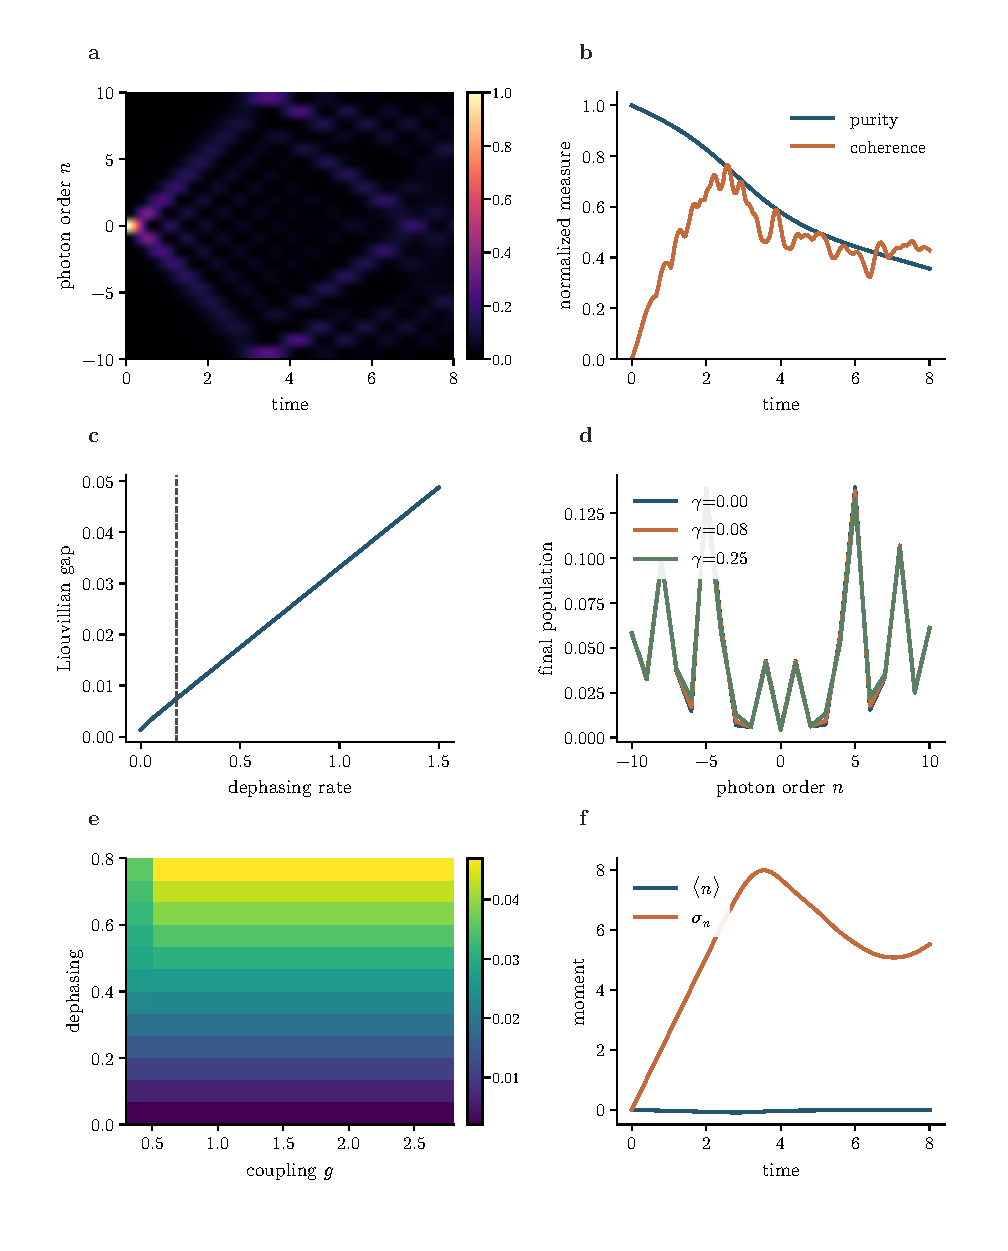
\includegraphics[width=0.96\linewidth,height=0.70\textheight,keepaspectratio]{open_system_quantum_walk.pdf}
\caption{\textbf{耗散 PINEM 能量晶格}\quad 这里的退相干率和弛豫率是有效马尔可夫参数。只有在环境关联时间短、系统—环境耦合弱时，才能把它们解释为微观环境关联函数导出的常数。 图中使用有限能量阶梯的 GKSL 模型，比较相干耦合、纯退相干和能量弛豫。人口传播给出边带怎样展开；由于初态是单格点纯态，能量基非对角元先由相干跃迁产生，随后才受环境破坏，不能将此曲线整体理解为单调退相干。纯度进一步刻画混合化，刘维尔谱隙则给出最慢耗散时间尺度。}
\label{fig:ch05-novel-extensions--11-open-system-quantum-walk}
\end{figure}

数值实现中，将有限能量阶梯 $n=-n_{\max},\ldots,n_{\max}$ 视为有效离散空间：
\[H=\Delta\sum_n n|n\rangle\langle n|+g\sum_{n=-n_{\max}}^{n_{\max}-1}\bigl(\ee^{\ii\varphi}|n+1\rangle\langle n|+\mathrm{h.c.}\bigr),\]
\[\dot\rho=-i[H,\rho]+\gamma_\phi\mathcal D[A_\phi]\rho+\gamma_r\mathcal D[A_r]\rho,\quad A_\phi=\sum_n\frac{n}{n_{\max}}|n\rangle\langle n|,\quad A_r=\sum_{n=-n_{\max}+1}^{n_{\max}}|n-1\rangle\langle n|,\]
\[\mathcal D[A]\rho=A\rho A^\dagger-\tfrac12\{A^\dagger A,\rho\},\qquad \mathcal P(t)=\operatorname{Tr}\rho(t)^2,\quad C(t)=\frac1{2n_{\max}}\sum_{n\ne m}|\rho_{nm}(t)|.\]
初态 $\rho(0)=|0\rangle\langle0|$，全程使用 $\Delta=0,\varphi=0$。主图 $g=1.8$、$n_{\max}=10$、$\gamma_\phi=0.18$、$\gamma_r=0.035$、$t\in[0,8]$（161 点）；谱隙图采用 $g=1.8,n_{\max}=4,\gamma_r=0.03$、$\gamma_\phi\in[0,1.5]$（41 点），$\mathrm{gap}=-\max_{\lambda\ne0}\operatorname{Re}\lambda(\mathcal L)$。终态比较 $\gamma_\phi=0,0.08,0.25$、$\gamma_r=0.02$、$t\in[0,5]$（101 点）；二维谱隙图 $g\in[0.3,2.8]$、$\gamma_\phi\in[0,0.8]$（各 12 点），$n_{\max}=3,\gamma_r=0.03$。最后一格绘制 $\langle n\rangle=\sum_n n\rho_{nn}$ 与 $\sigma_n=[\sum_n(n-\langle n\rangle)^2\rho_{nn}]^{1/2}$。$g,\Delta,\gamma_\phi,\gamma_r,t$ 均为无量纲唯象参数，不指代特定实验标定。


平均方程与单次探测记录的关系还可以直接数值检验。为避免把不同物理机制塞进同一个复杂晶格，先单独考虑一个被理想光子计数器连续监测的受驱动两能级发射体。这是通用 GKSL 理论的教学基准，不是把真实 PINEM 材料环境简化成一个已经证实的单光子发射器。取 $\hbar=1$，在 $\{|g\rangle,|e\rangle\}$ 上定义
\begin{equation}
 H=\frac{\Omega}{2}(|e\rangle\langle g|+|g\rangle\langle e|),\quad
 L=\sqrt{\Gamma}|g\rangle\langle e|,\quad
 H_{\rm eff}=H-\frac{\ii}{2}L^\dagger L .
 \label{eq:ch05-trajectory-heff}
\end{equation}
一次不发射的条件演化为未归一化的 $|\widetilde\psi(t+\delta t)\rangle=\ee^{-\ii H_{\rm eff}\delta t}|\psi(t)\rangle$；其范数平方正是这一小步没有探测到跃迁的概率。如果出现跃迁，则按 $L|\psi\rangle/\|L|\psi\rangle\|$ 更新到条件态。初态 $|g\rangle$ 的首个等待时间分布尤其简单：
\begin{equation}
 S(\tau)=\left\|\ee^{-\ii H_{\rm eff}\tau}|g\rangle\right\|^2,\quad
 w(\tau)=-\frac{\dd S}{\dd \tau}
 =\Gamma\left|\langle e|\ee^{-\ii H_{\rm eff}\tau}|g\rangle\right|^2 .
 \label{eq:ch05-waiting-density}
\end{equation}
受驱动的发射器刚完成一次发射后处于 $|g\rangle$，需要重新受驱动才会发射下一次光子，所以 $w(0)=0$，它不必是无记忆指数分布。多条计数记录中的跃迁时间也允许直接统计 $N_\gamma(T)$ 的方差，并与具有相同平均值的 Poisson 基准比较。无论单条记录多么跳跃不连续，只要使用同一个测量方案，所有条件态的系综平均就必须回到原来的 GKSL 结果。

\begin{figure}[!htbp]
\centering
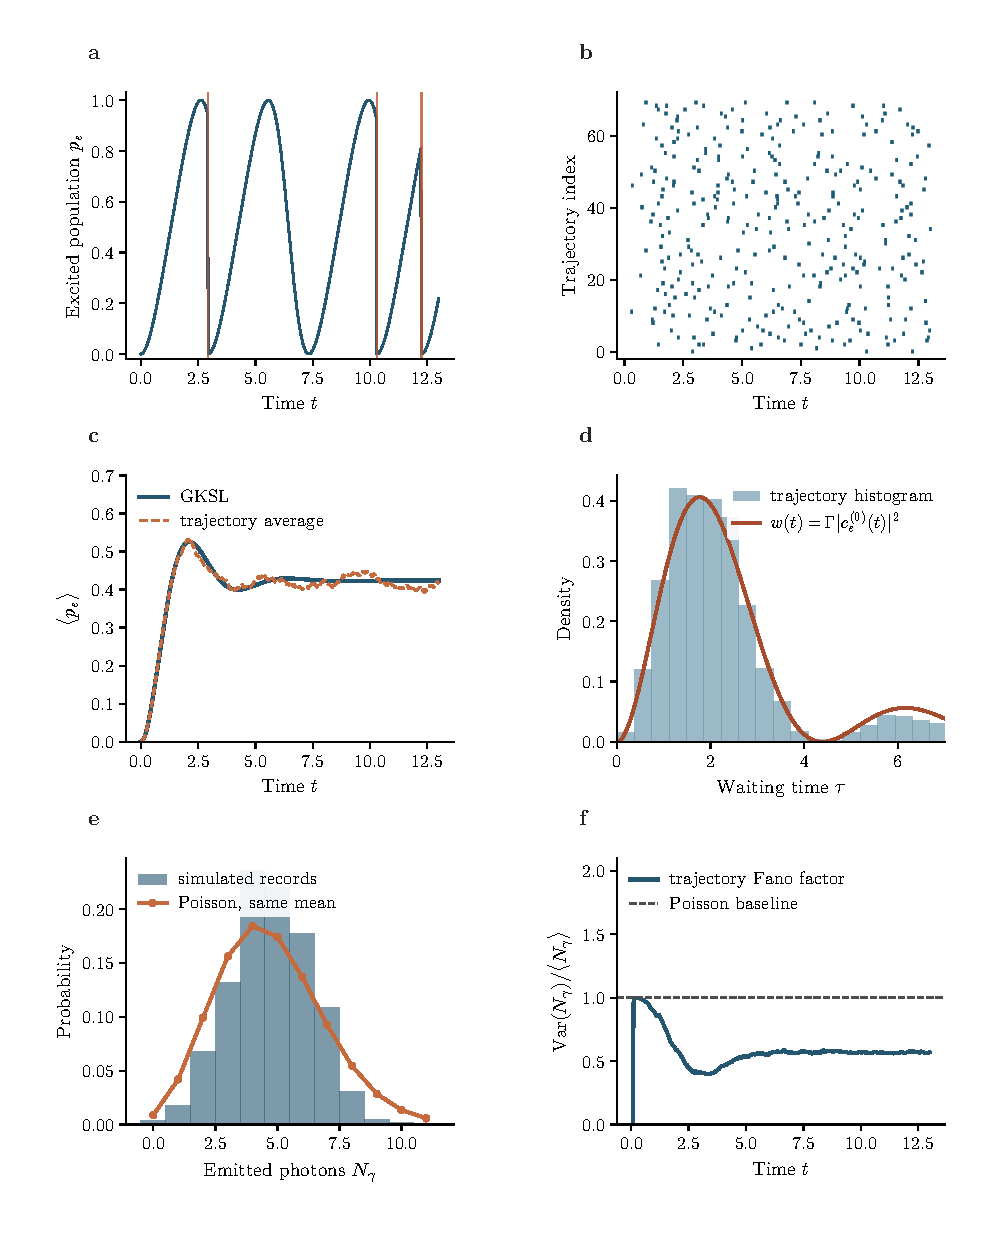
\includegraphics[width=0.96\linewidth,height=0.70\textheight,keepaspectratio]{quantum_jump_trajectories.pdf}
\caption{\textbf{从单次量子跳跃到平均主方程。} (a) 一条受驱动发射体的激发态条件人口，竖线表示光子跳跃；(b) 多次独立实验的跳跃时刻栅格；(c) 条件态平均与同一参数的 GKSL 方程直接对照；(d) 相邻跃迁的等待时间分布与无跳跃传播的解析预测比较；(e) 固定观察时间的发射光子数分布与同均值 Poisson 基准比较；(f) 用 $\operatorname{Var}N_\gamma/\langle N_\gamma\rangle$ 衡量随时间变化的计数涨落。这里的“探测记录”来自声明过的理想跳跃算符，不把它直接等同于电子能量损失探测器的点击信号。}
\label{fig:ch05-quantum-jump-trajectories}
\end{figure}

数值实现中，各格均基于\cref{eq:ch05-trajectory-heff}，以 $\Omega=1.5$、$\Gamma=0.9$、$\hbar=1$，初始条件 $|g\rangle$、无失谐和无额外纯退相干。单次演化以 $\delta t=0.026$、$500$ 步模拟至 $T=13$，每步先使用精确的非厄米矩阵指数 $M=\ee^{-\ii H_{\rm eff}\delta t}$，以 $1-\|M\psi\|^2$ 为跳跃概率并做条件归一化，发生跳跃时状态置为 $|g\rangle$；采用 $850$ 条独立蒙特卡洛记录，伪随机种子 $20261009$。(a) 显示第 $1$ 条轨迹条件激发人口和对应跳跃时刻；(b) 显示前 $70$ 条记录的全部光子点击；(c) 将 $850$ 条轨迹在每个时间点的 $|\langle e|\psi\rangle|^2$ 平均，与 $\dot\rho=-\ii[H,\rho]+\Gamma\mathcal D[|g\rangle\langle e|]\rho$ 的高精度常微分方程解比较；(d) 以 $35$ 个宽度相同的直方箱覆盖等待时间 $[0,13]$，叠加 $w(\tau)=\Gamma|\langle e|\ee^{-\ii H_{\rm eff}\tau}|g\rangle|^2$。有限观察窗带来右删失，尾部直方图因此会受采样偏差影响。(e) 在 $T=13$ 按轨迹计数 $N_\gamma$，用同样均值的 Poisson 分布作基准；(f) 用样本方差（自由度 $849$）与样本均值形成 Fano 因子，并画 $F=1$ 的 Poisson 基线。除采样随机性外不再引入任意背景或检测效率参数；时间、频率和速率均为同一无量纲模型单位。


从这张图再回到电子能量晶格，就能明确两种不同的实验要求：若只要无条件能谱，主方程或量子通道已经足够；若想利用每一次损失事件的实际时间或类型进行反馈，就需要说明监测了哪些环境通道以及探测效率是多少。对未被监测的材料模式，单条“量子轨迹”只是计算展开，并不自动对应可取得的实验记录。


控制电子或光场的相位与幅度，相当于直接设计 $H(t)$ 中的可调项。一个只在标称参数点达到单位保真度的脉冲往往很脆弱；更有意义的是在失谐、脉冲面积和退相干率存在小范围误差时仍维持较高保真度。因此，鲁棒控制应比较高保真区域在参数空间中的宽度，而不能只寻找一个孤立的最高点。

\begin{figure}[!htbp]
\centering
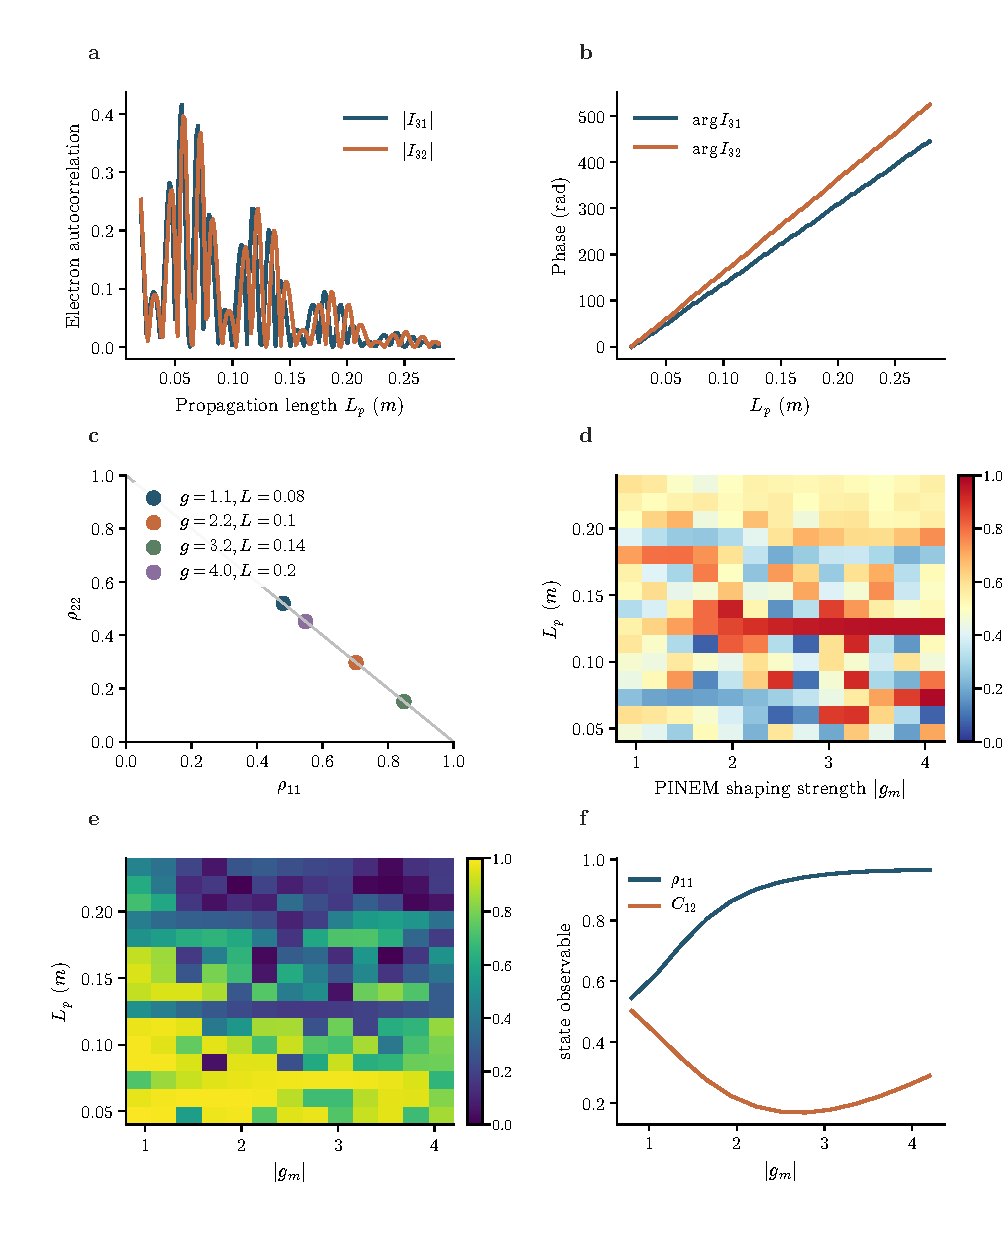
\includegraphics[width=0.96\linewidth,height=0.70\textheight,keepaspectratio]{wu2026_shaped_electron_control.pdf}
\caption{\textbf{整形电子相干控制}\quad 整形电子把入射波包的能量分量和相位变成可控变量。不同能量分量到达原子或量子系统时，可以沿不同跃迁路径驱动同一末态，因此电子自身的谱相位会进入系统的干涉项。图先用电子自相关刻画可用的相干时间结构，再比较人口与非对角相干随控制参数和时间的变化；在开放系统中，这些相干项还会与弛豫和退相干竞争。}
\label{fig:ch05-theory-atlas--14-wu2026-shaped-electron-control}
\end{figure}

数值实现中，整形电子的纵向相关函数按归一化双边带波包重叠计算：
\[I(u;g_m,L_p)=\frac{\int \dd q\,\psi_{g_m,L_p}(q+u)\psi^*_{g_m,L_p}(q)}{\int \dd q\,|\psi_{g_m,L_p}(q)|^2},\qquad u_{3j}=\omega_{3j}/v_0,\]
\[\mathcal F=e^{\mathcal L T_{\rm rep}}\mathcal S[I],\qquad \mathcal F(\rho_{\rm ss})=\rho_{\rm ss},\qquad C_{12}=\min\!\left(1,\frac{|\rho_{12}|}{\sqrt{\rho_{11}\rho_{22}}}\right).\]
其中 $\mathcal S$ 包括一次和二次电子散射矩阵元，$\mathcal L$ 由辐射跃迁与纯退相干 Lindblad 项构成；$\psi$ 是权重 $J_n(2|g_m|)$、宽度 $\sigma_q$ 的高斯边带波包，并使用二阶纵向色散相位 $D=\hbar/(2\gamma_0^3m_ev_0)$。所采用的具体唯象数值为 $v_0=0.5c$，$\gamma_0=(1-0.5^2)^{-1/2}$，$\sigma_q=10^6\,\mathrm{m}^{-1}$，$\omega_{\rm PINEM}=1.5\times10^{15}\,\mathrm{s}^{-1}$，源区长度 $L_s=0.100\,\mathrm m$，重复周期 $T_{\rm rep}=0.5\,\mathrm{ns}$，冲量参数 $b=1\,\mathrm{nm}$；$\omega_{31}=3.0\times10^{15}\,\mathrm{s}^{-1}$、$\omega_{32}=2.9\times10^{15}\,\mathrm{s}^{-1}$，$d_{31}=2.16\times3.33564\times10^{-30}\,\mathrm{C\,m}$、$d_{32}=2.03\times3.33564\times10^{-30}\,\mathrm{C\,m}$，三态纯退相干输入数组 $(0.95\times10^3,1.0\times10^3,2.0\times10^6)\,\mathrm{s}^{-1}$；自发辐射率按 $\Gamma_{3j}=\omega_{3j}^3d_{3j}^2/(3\pi\varepsilon_0\hbar c^3)$ 给定。边带求和截断 $n_{\max}=\max\{12,\lceil2|g_m|+10\rceil\}$。
图 (a,b) 固定 $g_m=2.2$、$L_p\in[0.02,0.28]\,\mathrm m$（220 点）；(c) 的 $(g_m,L_p)$ 为 $(1.1,0.08),(2.2,0.10),(3.2,0.14),(4.0,0.20)$；(d,e) 取 $g_m\in[0.8,4.2]$（13 点）、$L_p\in[0.04,0.24]\,\mathrm m$（15 点）；(f) 是最接近 $L_p=0.12\,\mathrm m$ 的栅格截面。图 (e,f) 画的是归一化相干性 $C_{12}$，不是未归一化矩阵元 $|\rho_{12}|$。这些参数是该数值重建模型的指定设置，不应解读为普适实验常数。

图 (a) 给出两个跃迁频率上的谱自相关模，(b) 将同一复自相关的辐角连续展开，避免把 $2\pi$ 支切误读成相位突变；(c) 比较前述四组驱动参数求得的三能级固定点 $\rho_{\rm ss}$；(d,e) 在相同的 $13\times15$ 参数网格上分别显示布居 $\rho_{11}$ 与归一化相干性 $C_{12}$，(f) 为 $L_p$ 最接近 $0.12\,\mathrm m$ 的截面。计算中的跃迁率、纯退相干和截断均取上文给出的数值，不能将这组唯象参数解读成已标定的实验条件。


前面的主方程说明环境怎样改变系统态。Wu 等的工作进一步把一个整形自由电子脉冲看成可重复的量子驱动：电子先由 PINEM 与自由漂移获得可调自相关，再与三能级体系散射，最后在相邻电子之间按开放系统动力学演化。

Wu 等把这一过程写成周期重复的量子映射，使整形电子从“一次散射探针”变成可积累的相干驱动器。\textsuperscript{\hyperref[ch05-ref1]{[1]}}
论文先写整形电子本身。电子经过 PINEM 调制和两段自由传播后，动量波函数是多个贝塞尔加权的能量分量叠加；真正控制三能级跃迁的是电子自相关 $I(u)=\int \dd q\,\psi_e(q+u)\psi_e^*(q)$。漂移长度 $L_p$ 改变不同能量分量的相对相位，所以它能连续调节两个跃迁通道的复振幅。

电子与 $\Lambda$ 型三能级体系的相互作用从 库仑偶极哈密顿量出发。论文参数给出无量纲耦合 $|G_{ij}|\sim10^{-3}$，因此把单电子散射矩阵保留到二阶是受控的。每个电子散射后先对电子自由度取迹，得到三能级密度矩阵的离散更新；两次电子之间再按含自发辐射和纯退相干的 Lindblad 方程演化。

于是一个周期的动力学是固定线性映射 $F=L(I+D)$，稳态满足 $v_{ss}=Fv_{ss}$。论文图 2、3 扫描 $|g_m|$ 和 $L_p$ 得到人口与低能级相干度的干涉条纹；两种能级配置的跃迁频率比不同，所以条纹周期也不同。最后图 4 从具体参数点做时间演化，验证系统从任意初态收敛到高相干或完全人口转移的暗态。


把整形电子用于三能级控制时，最容易写得过快的一步，是直接把它类比成两束激光驱动的 $\Lambda$ 系统。论文真正做的事情更具体：先用 PINEM 制备具有离散能量梳和可控谱相位的电子波包，再让单个电子通过库仑相互作用同时耦合 $|1\rangle\leftrightarrow|3\rangle$ 与 $|2\rangle\leftrightarrow|3\rangle$ 两条跃迁，最后把重复电子脉冲看成周期量子驱动，并在两次电子到来之间加入耗散。\textsuperscript{\hyperref[ch05-ref1]{[1]}}

整形电子的自由传播并不是无关紧要的延迟。PINEM 后第 $n$ 个能量分量在漂移长度 $L_p$ 上积累色散相位，所以到达三能级系统时，不同 $n$ 的相对相位由 $g_m$ 和 $L_p$ 共同控制。对一个给定跃迁频率 $\omega_{ij}$，电子驱动强度可以抽象成波包的能量自相关
\begin{equation}
C_e(\omega_{ij})=\int\dd  q\,\psi^*(q)\psi\!\left(q+\frac{\omega_{ij}}{v_0}\right),
\label{eq:ch05-electron-autocorr}
\end{equation}
它衡量相差一个跃迁能量的电子分量之间是否同时存在且保持相干。未整形电子若能量宽度远小于 $\hbar\omega_{ij}$，这个重叠很小；PINEM 能量梳则可以人为制造所需的相干间隔。

对论文参数，单电子--三能级耦合仍处于弱散射区，因而每次碰撞可用二阶 $S$ 矩阵展开。真正的强控制来自\emph{许多弱碰撞的相干重复}，而不是单个电子一次把布居完全翻转。若把一次电子碰撞得到的量子映射记为 $\mathcal E_e$，两电子间隔 $T$ 内的耗散映射记为 $\mathcal E_d(T)$，则一周期演化为
\begin{equation}
\rho_{k+1}=\mathcal E_d(T)\circ\mathcal E_e[\rho_k].
\label{eq:ch05-stroboscopic-map}
\end{equation}
稳定态满足 $\rho_*=\mathcal E_d\circ\mathcal E_e[\rho_*]$。因此论文所说“稳定态与初态无关”在数学上对应这个离散量子通道具有唯一吸引不动点，而不是简单因为时间足够长。

暗态的物理也可以直接从两条跃迁路径读出。若有效电子驱动在两条跃迁上的复振幅分别为 $\Omega_{31}^{(e)}$ 和 $\Omega_{32}^{(e)}$，则与激发态解耦的线性组合满足
\begin{equation}
|D\rangle\propto \Omega_{32}^{(e)}|1\rangle-\Omega_{31}^{(e)}|2\rangle,
\label{eq:ch05-dark-state}
\end{equation}
因为 $\langle3|H_{\rm drive}|D\rangle=0$。PINEM 耦合强度和漂移长度改变的是 $\Omega_{31}^{(e)}/\Omega_{32}^{(e)}$ 的幅度与相位，所以它们移动暗态在两个低能级之间的组成。所谓电子介导的相干布居俘获，本质上就是利用整形电子把这个比值调到使两条激发路径相消的位置。

这样的相消对相位稳定度提出了可以量化的要求。记两条有效跃迁振幅的模为 $A=|\Omega_{31}^{(e)}|$ 和 $B=|\Omega_{32}^{(e)}|$，相对相位为 $\phi$。将归一化暗态写成 $|D(\phi)\rangle=[B\ee^{\ii\phi}|1\rangle-A|2\rangle]/\sqrt{A^2+B^2}$，一次随机相位漂移 $\delta\phi$ 后的暗态重叠概率是
\begin{align*}
|\langle D(\phi)|D(\phi+\delta\phi)\rangle|^2
&=\frac{A^4+B^4+2A^2B^2\cos\delta\phi}{(A^2+B^2)^2}\\
&=1-\frac{2A^2B^2}{(A^2+B^2)^2}(1-\cos\delta\phi).
\end{align*}
若相位噪声服从零均值高斯分布，方差为 $\sigma_\phi^2$，用 $\langle\cos\delta\phi\rangle=\ee^{-\sigma_\phi^2/2}$ 可直接得到平均暗态保真度
\begin{equation}
\overline{F}_D=1-\frac{2A^2B^2}{(A^2+B^2)^2}
(1-\ee^{-\sigma_\phi^2/2}).
\label{eq:dark-state-phase-jitter}
\end{equation}
等幅度驱动 $A=B$ 且 $\sigma_\phi\ll1$ 时，暗态泄漏为 $1-\overline F_D\simeq\sigma_\phi^2/4$。这一结果讨论的是相位平均造成的失配，不自动包含材料耗散或非马尔可夫记忆。它把“暗态需要相位稳定”转化成一个可以代入光学相位噪声谱和漂移抖动的实验量，而不是附加的经验衰减常数。

从研究角度看，下一步最值得检查的不是继续增加能级数，而是先破坏论文的理想条件：若两跃迁偶极矩不平行、电子冲击参数有分布、到达时间有抖动，或 $C_e(\omega)$ 在两个跃迁频率处的相位不稳定，\cref{eq:ch05-dark-state} 的相消会变成不完全相消。把这些噪声直接写进\cref{eq:ch05-stroboscopic-map}，计算稳定态保真度对实验分布的函数，比单独画理想布居图更接近一个可以继续发表的鲁棒控制问题。

有了可控散射路径，剩下的难题就不再是找到单个理想脉冲，而是理解这些干涉路径对失谐、相位噪声和耗散的响应。因而下面回到噪声谱与控制滤波的共同语言。
同样的噪声均方根幅度可以产生完全不同的退相干，因为系统只对控制序列允许通过的频率敏感。设随机扰动为 $\delta\lambda(t)$，其功率谱密度为 $S(\omega)$；控制序列把噪声耦合调制成频率响应 $F(\omega,T)$。在弱高斯噪声近似下，相干包络常可写成 $\mathcal C(T)=e^{-\chi(T)}$，其中 $\chi$ 是 $S$ 与 $F$ 的重叠积分。

因此鲁棒控制不是单纯增大驱动，而是让滤波函数的主要权重避开噪声谱峰。若噪声强到高阶累积量不可忽略，或环境具有明显非高斯统计，单一滤波函数描述会失效，此时应回到随机哈密顿量或非 Markov 主方程。


只保留纯退相干，取 $L=\sigma_z$，并把对应速率记为 $\gamma_\phi/2$。把密度矩阵写成 $\rho_{ij}$，代入 GKSL 方程可得对角元不变，而非对角元满足


\begin{equation*}
\dot\rho_{12}=-\gamma_\phi\rho_{12},\qquad \rho_{12}(t)=\rho_{12}(0)e^{-\gamma_\phi t}.
\end{equation*}


所以纯退相干可以在短时间内保持能级人口，却把相位信息指数洗掉。若再加入拉比驱动 $H=\hbar\Omega\sigma_x/2$，相干旋转的时间尺度是 $1/\Omega$，环境破坏相干的时间尺度是 $1/\gamma_\phi$。两者的竞争只取决于无量纲比值 $\gamma_\phi/\Omega$。

因此后面的控制图横纵轴使用 $\gamma/\Omega$、$\Delta/\Omega$ 等比值是有直接物理意义的：当这些比值远小于 1 时，系统来得及完成相干旋转；当它们接近或超过 1 时，退相干或失谐会在一个控制周期内积累到不可忽略。

把失谐和退相干率都除以典型拉比频率 $\Omega$，可得到普适的参数平面 $(\Delta/\Omega,\gamma/\Omega)$。当这两个比值都小于 1 时，相干旋转通常仍占主导；当退相干快于控制时，振荡被压低并进入过阻尼或 Zeno 区。


刘维尔模、有色噪声、复合脉冲和 Zeno 交叉都在检验同一个问题：环境时间尺度与控制时间尺度接近时，哪一个理想结论首先失效。把这些结果放在一起，可以区分“模型本身失效”和“控制参数选得不好”。

\begin{figure}[!htbp]
\centering
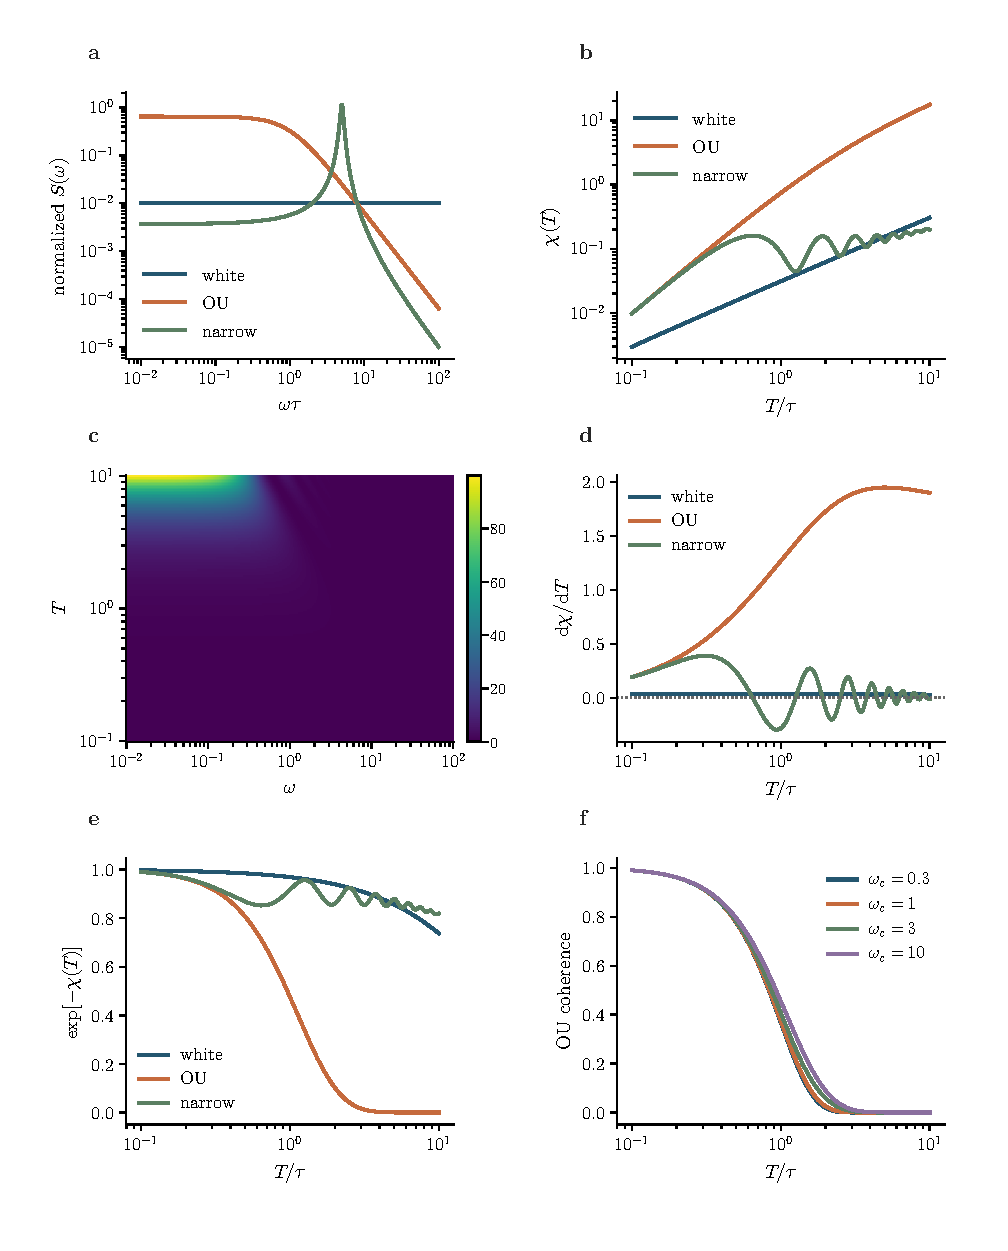
\includegraphics[width=0.96\linewidth,height=0.70\textheight,keepaspectratio]{noise_spectrum.pdf}
\caption{\textbf{有色噪声谱与滤波函数}\quad 白噪声、Ornstein--Uhlenbeck 噪声和窄带噪声可以具有相同均方根幅度，却在频域中分布完全不同。控制序列的滤波函数决定哪些频率真正进入退相干积分，因此相干损失取决于谱重叠，而不是只取决于一个噪声幅度。}
\label{fig:ch05-story-extensions--29-noise-spectrum}
\end{figure}

对同一控制滤波函数计算噪声谱重叠，不再混用人为指定的指数曲线：
\[\begin{aligned}
S_{\rm w}(\omega)&=1,\quad S_{\rm OU}(\omega)=\frac1{1+\omega^2},\quad S_{\rm n}(\omega)=\frac{0.08}{(\omega-5)^2+0.08},\\
\chi_s(T)&=\frac{\displaystyle\int_{\omega_-}^{\omega_+}\dd \omega\,S_s(\omega)\,4\sin^2(\omega T/2)/\omega^2}{\displaystyle\int_{\omega_-}^{\omega_+}\dd \omega\,S_s(\omega)}.
\end{aligned}\]
取 $\omega\in[10^{-2},10^2]$（500 对数点）、$T\in[0.1,10]$（180 对数点），并显示 $e^{-\chi_s(T)}$。第四子图直接取同一时间网格上的数值微分 $\gamma_{\rm eff}(T)=\dd \chi_s/\dd  T$，在固定初始时刻观察到的负率不代表 $\chi_s<0$。第六子图对 OU 谱取积分上限 $\omega_c=0.3,1,3,10$，每条曲线采用相同总谱面积归一化。频率与时间均无量纲；未在图中引入与 $S_s$ 无关的唯象退相干率。

具体到各面板，(a) 在 $\omega=10^{-2}$--$10^2$ 的 500 个对数采样点上绘 $S_s(\omega)/\int S_s\dd \omega$，$s=$ white、OU、窄带；(b) 对相同三谱作 $\chi_s(T)=\int S_s F_T\dd \omega/\int S_s\dd \omega$，其中 $F_T=4\sin^2(\omega T/2)/(\omega^2+10^{-12})$；(c) 直接画该滤波核 $F_T$ 的 $\omega$--$T$ 分布；(d) 在同一离散时间网格对 $\chi_s(T)$ 使用 \texttt{numpy.gradient(vals,T)} 求瞬时有效退相干率 $\gamma_{\rm eff}(T)=\dd \chi_s/\dd  T$，没有另拟合一个马尔可夫常数；若窄带谱出现短时负率，应解释为非马尔可夫回流而非负总噪声功率；(e) 从 (b) \emph{不添加新退相干常数}算 $e^{-\chi_s(T)}$；(f) 仅对 OU 谱重复积分，逐个采用截断 $\omega_c=0.3,1,3,10$ 并在保留区间重新归一化，画 $e^{-\chi_{\rm OU}(T;\omega_c)}$。这里三谱以\emph{单位积分}固定噪声面积，白噪声的积分值依赖规定的有限带宽。


\medskip

前图比较的是不同经验谱经过同一个滤波核后的响应，仍有一个值得完整推导的可解模型：即使把噪声均方根保持不变，仅仅改变相关时间，最有效的实验控制序列也可能发生变化。使用具有指数关联的经典高斯 Ornstein--Uhlenbeck 相位噪声，可以把这个问题从哈密顿量一直算到回波对比度，而不需要额外给每一幅图引入独立的“有效退相干率”。

令两能级的随机频率偏移通过 $H_\xi(t)=\xi(t)\sigma_z/2$ 耦合，$\langle\xi(t)\rangle=0$，并令相关函数为
\begin{equation}
C(\tau)=\langle\xi(t)\xi(t+\tau)\rangle
=\sigma_\xi^2e^{-|\tau|/\tau_c},\qquad
S(\omega)=\int_{-\infty}^{\infty}\!\dd \tau\,C(\tau)\ee^{\ii\omega\tau}
=\frac{2\sigma_\xi^2\tau_c}{1+\omega^2\tau_c^2}.
\label{eq:ch05-ou-spectrum}
\end{equation}
$\sigma_\xi$ 的量纲是角频率，$\tau_c$ 是相关时间。自由演化下的相位积累为 $\Phi(T)=\int_0^T\xi(t)\,\dd t$。若在时间 $T/2$ 理想施加一个瞬时 $\pi$ 脉冲，噪声耦合符号在脉冲两侧翻转，条件相位就变成 $\Phi_y(T)=\int_0^T y(t)\xi(t)\,\dd t$，其中自由演化 $y_{\rm FID}=1$，Hahn 回波的 $y_{\rm E}=+1$（前半段）和 $-1$（后半段）。

由于噪声为零均值高斯过程，累积量展开在二阶严格闭合，从而得到
\begin{equation}
W_y(T)=\left\langle \ee^{-\ii\Phi_y(T)}\right\rangle
=e^{-\chi_y(T)},\quad
\chi_y=\frac12\int_0^T\!\dd t\int_0^T\!\dd t'\,
 y(t)y(t')C(t-t')
=\frac1{4\pi}\int_{-\infty}^{\infty}\!\dd \omega\,S(\omega)|Y_T(\omega)|^2,
\label{eq:ch05-filter-functional}
\end{equation}
其中 $Y_T(\omega)=\int_0^T y(t)\ee^{\ii\omega t}\,\dd t$。这一步精确展示了“噪声谱”和“脉冲控制序列”的分工：材料与技术环境决定 $S$，控制脉冲只决定 $Y_T$，两者相乘积分才构成退相干指数。对同一个 OU 过程，两个序列的解析解恰好为
\begin{equation}
\begin{aligned}
\chi_{\rm FID}(T)&=\sigma_\xi^2\tau_c^2\left[\frac{T}{\tau_c}-1+e^{-T/\tau_c}\right],\\
\chi_{\rm E}(T)&=\sigma_\xi^2\tau_c^2\left[\frac{T}{\tau_c}-3+4e^{-T/(2\tau_c)}-e^{-T/\tau_c}\right].
\end{aligned}
\label{eq:ch05-ou-exact}
\end{equation}
短时展开得到 $\chi_{\rm FID}\simeq\sigma_\xi^2T^2/2$、$\chi_{\rm E}\simeq\sigma_\xi^2T^3/(12\tau_c)$。所以回波并不是“让退相干率降低一个恒定倍数”，而是在慢变噪声下抵消主导的二次相位误差。若 $\tau_c$ 很短，脉冲前后的随机相位基本独立，回波的优势就大幅减弱。

\begin{figure}[!htbp]
\centering
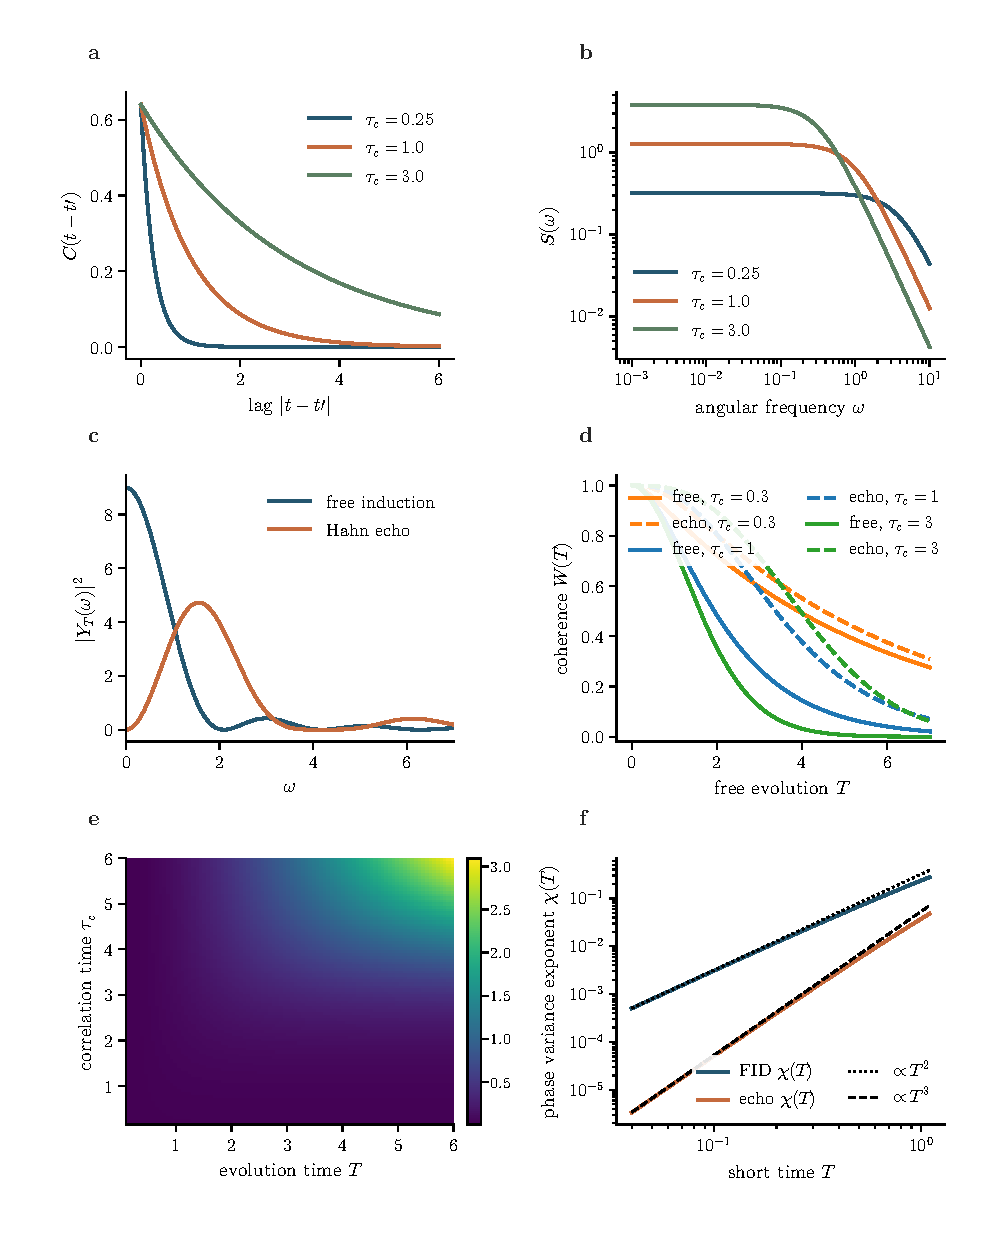
\includegraphics[width=0.97\linewidth,height=0.70\textheight,keepaspectratio]{colored_noise_echo.pdf}
\caption{\textbf{从有色噪声谱推导自由感应衰减与 Hahn 回波}\quad (a) 不同相关时间的指数型噪声协方差；(b) 其解析双边 Lorentz 谱；(c) 自由演化和理想 Hahn 回波在相同总作用时间下的滤波函数；(d) 从同一个 OU 相关函数计算的相干对比度，两种控制序列不再共享一个经验衰减常数；(e) 在传播时间与相关时间平面上的回波提升因子；(f) 用双对数坐标直接检验自由衰减的 $T^2$ 和回波的 $T^3$ 短时标度。所有曲线都由同一解析高斯模型生成，并以谱域积分作独立核查。}
\label{fig:ch05-colored-noise-echo}
\end{figure}

使用\cref{eq:ch05-ou-spectrum,eq:ch05-ou-exact}，噪声均方根幅度固定 $\sigma_\xi=0.8$；(a) 绘 $\tau\in[0,6]$ 的协方差，取 $\tau_c=0.25,1,3$，每条曲线同起点 $C(0)=0.64$；(b) 绘相同相关时间、正频率 $\omega\in[10^{-3},10]$ 的双边谱密度 $S(\omega)$，不把单边谱和双边谱混用。(c) 固定 $T=3$，绘 $\omega\in[10^{-3},10]$ 上的 $|Y_T|^2$，使用 $|Y_{\rm FID}|^2=4\sin^2(\omega T/2)/\omega^2$ 和 $|Y_{\rm E}|^2=16\sin^4(\omega T/4)/\omega^2$。(d) 用\cref{eq:ch05-ou-exact} 计算 $T\in[0,7]$（450 点）、$\tau_c=0.3,1,3$ 时的两类对比度 $W=e^{-\chi}$。(e) 在 $\tau_c\in[0.15,6]$ 的 90 个对数点与 $T\in[0.1,6]$ 的 90 个线性点上绘 $\log_{10}(W_{\rm E}/W_{\rm FID})$，色阶来自同一解析式，不再独立归一化。(f) 固定 $\tau_c=1$，在 $T\in[0.04,1.1]$ 的 120 个对数点比较 $\chi_{\rm FID}$、$\chi_{\rm E}$ 与各自 $\sigma_\xi^2T^2/2$、$\sigma_\xi^2T^3/(12\tau_c)$ 的渐近标度。代码另在 $\omega\in[10^{-5},350]$ 上取 250000 点进行正频率积分 $\chi=\int_0^\infty\!\dd \omega\,S(\omega)|Y_T|^2/(2\pi)$，并检验 $T=3,\tau_c=1$ 的解析结果；这一步只是数值核查，不引入额外图示参数。忽略 $\pi$ 脉冲宽度、退相干通道之间的相关性及高斯过程以外的高阶累积量。


这也提示了实验判据的严格程度。单凭对比度出现衰减，不能断言处于 Markov 主方程；同样，看到回波改善并不意味着存在非经典环境。这里的 OU 噪声是经典高斯随机过程，已经能够生成明显的记忆效应。真实材料中的非高斯涨落、环境反作用或有限宽度控制脉冲会修正\cref{eq:ch05-ou-exact}；一旦这些效应显著，应该回到双时刻相关函数甚至更高阶关联，而不是悄悄重新拟合一个时间依赖的 $\gamma_\phi$。

相干驱动、能量弛豫、纯退相干和控制误差作用在不同时间尺度上。把它们放在同一组无量纲坐标中，可以直接判断控制失败究竟来自失谐、退相干还是脉冲本身对参数扰动过于敏感。


\medskip
GKSL 方程不是从幺正动力学“直接得到”的，而是在弱系统--环境耦合、短环境记忆和适当频率分离条件下，由总体系动力学逐步约化得到。

弛豫和纯退相干对人口与相干性的作用不同；对两能级模型，$T_2$ 同时受 $T_1$ 和纯退相干率限制，因此只测人口不足以确定相干寿命。

滤波函数、复合控制和整形电子驱动都可以理解为改变系统对噪声频谱或跃迁路径的权重，但现象学控制评分不能替代具体系统--浴模型。

Wu 等 2026 的正式论文把整形自由电子列作为周期量子驱动器，用于三能级相干俘获和稳态控制；该结果与本章前面的开放系统框架在稳态 Lindblad 演化处衔接。

环境能够改变单电子相干性，而且 2026 年的材料理论已经把这种衰减从单一现象学速率推进到依赖材料激发谱、温度和路径几何的非局域核；但环境仍不是联合信号的唯一来源。两个不可分辨电子之间还存在交换结构，下文将把交换效应与真实两体相互作用分开。

\clearpage
\par\medskip 把闭系相干调制升级成开放系统时，必须写出环境怎样作用在格点基底上。对角跳跃算符主要抑制非对角相干；能量降阶算符既改变人口也改变相干。此处的 Lindblad 率和演化时间只定义无量纲数值实验，图中的 $t=5$ 截面不代表已达到稳态，只有求解 $\mathcal L\rho_{\rm ss}=0$ 并检验收敛后才能使用稳态一词。


\noindent \figref{fig:ch05-novel-extensions--11-open-system-quantum-walk}：六面板计算逐项核对。\par\noindent (a) 对初态 $|0\rangle\langle0|$ 数值积分 $\exp(t\mathcal L)$ 并绘 $\rho_{nn}(t)$，$n=-10,\ldots,10$；(b) 从同一密度矩阵计算 $\operatorname{Tr}\rho^2$ 及 $\sum_{n\ne m}|\rho_{nm}|/(2n_{\max})$；(c) $n_{\max}=4$、$g=1.8$、$\gamma_r=0.03$，在 $\gamma_\phi=0$--$1.5$ 的 41 点取 Liouvillian 非零实部衰减率；(d) 只在 $t=5$ 比较 $\gamma_\phi=0,0.08,0.25$，$\gamma_r=0.02$，不是稳态；(e) 用更小的 $n_{\max}=3$ 求 $12\times12$ 格点上的谱隙，$g\in[0.3,2.8]$、$\gamma_\phi\in[0,0.8]$；(f) 与 (a) 同态计算 $\langle n\rangle$ 和 $\sqrt{\langle n^2\rangle-\langle n\rangle^2}$。所有时间、频率、退相干率都是无量纲；(c,e) 的不同截断不能混称同一个有限尺寸体系。


\par\medskip
环境偏迹解释了单电子相干为何衰减，但联合电子计数还涉及另一种来源：不可分辨费米子的交换反对称性。下面先将交换效应与真实粒子间相互作用分开，再讨论探测器中的二电子关联；二者不能仅凭能谱上的反相关外形互相替代。
\par\medskip


\section{交换与碰撞}
两个电子的联合计数出现关联，并不自动说明电子之间发生了强库仑散射。即使把粒子间势完全关掉，只要两个电子不可分辨，费米反对称性就已经会改变联合概率。因此必须先把“交换造成的关联”和“相互作用在演化中产生的关联”分开。

设两个归一化单粒子轨道为 $\phi_a$、$\phi_b$，重叠为 $S=\langle\phi_a|\phi_b\rangle$。对平行自旋电子，空间波函数必须反对称：

\begin{equation}
\Psi_A(1,2)=\frac{\phi_a(1)\phi_b(2)-\phi_b(1)\phi_a(2)}{\sqrt{2(1-|S|^2)}},\qquad |S|<1.
\label{eq:ch06-1}
\end{equation}

归一化因子来自两项交换振幅的内积：未归一化分子范数平方为 $2(1-|S|^2)$。当 $|S|=1$ 时，两轨道线性相关，反对称组合恒为零，不能据此构造双电子态。\cref{eq:ch06-1} 的第二项来自粒子交换，并非额外相互作用。两项在概率中产生交叉项，所以即使 $V=0$，联合计数也一般不能写成两个独立单粒子概率的乘积。

真实动力学关联来自两体哈密顿量

\begin{equation}
H=h(1)+h(2)+V(\vb{r}_1-\vb{r}_2),\qquad V_C(r)=\frac{e^2}{4\pi\varepsilon_0 r}\ \text{（真空库仑势）}.
\label{eq:ch06-2}
\end{equation}

$h(i)$ 包含第 $i$ 个电子的自由传播和外场耦合。若考虑介质屏蔽、边界或延迟效应，$V$ 必须换成相应的有效相互作用，不能继续使用真空库仑势。与交换不同，$V$ 会在时间演化中改变双体态本身；即使初态只有一个 Slater 行列式，演化后也可能需要多个 Slater 组态才能表示。

若先采用有序的双粒子通道标签 $n_1,n_2$，并在相应反对称子空间中定义密度矩阵，联合概率与连通关联可记为

\begin{equation}
P(n_1,n_2)=\langle n_1,n_2|\rho_{12}|n_1,n_2\rangle,\qquad C(n_1,n_2)=P-P_1P_2.
\label{eq:ch06-3}
\end{equation}

若实验只记录无序的两电子结果，还须对 $(n_1,n_2)$ 与 $(n_2,n_1)$ 的计数作相应合并，避免重复计数。连通关联 $C$ 表示联合概率相对于边缘分布乘积的偏离，本身不能识别该偏离来自交换还是相互作用 $V$。要分辨来源，必须额外改变可分辨性，例如相对延迟或自旋，再独立改变相互作用强度或作用时间。只有两类扫描给出不同响应，才有可能把两种机制分开。

对于不可分辨费米子，普通的粒子 Schmidt 分解容易把反对称性本身误算成纠缠。更稳妥的做法是检查单粒子约化密度矩阵的自然占据数或 Slater 秩，并明确采用的“费米子纠缠”定义。后文凡使用 施密特（Schmidt）数的简化图，只把它当作相关维数的模型指标，不把它直接等同于可操作的双电子纠缠度量。

为了看清库仑势实际作用在哪个自由度上，先忽略外场的不均匀性，并取两个电子质量都为 $m_e$。定义质心坐标 $\vb{R}=(\vb{r}_1+\vb{r}_2)/2$ 和相对坐标 $\vb{r}=\vb{r}_1-\vb{r}_2$，相应动量为 $\mathbf P=\vb{p}_1+\vb{p}_2$、$\vb{p}=(\vb{p}_1-\vb{p}_2)/2$。自由动能严格分解为

\begin{equation}
\frac{p_1^2}{2m_e}+\frac{p_2^2}{2m_e}=\frac{P^2}{4m_e}+\frac{p^2}{m_e}.
\label{eq:ch06-4}
\end{equation}

若外场在两电子间距上变化很慢，它主要共同推动质心；而 $V(\vb{r})$ 只进入相对运动。于是“两个电子一起被光场加速”和“两个电子彼此改变相对动量”在最低阶可以分开。若两电子相距已经与近场变化尺度相当，这个分离不再成立，外场梯度本身也会驱动相对运动。

若 PINEM 或 Kapitza--Dirac 场分别对两个电子实施单粒子幺正变换 $U\otimes U$，它不会改变双体态中由相互作用产生的总关联量，但会改变这些关联在能量、动量或 OAM 基中的分布。换句话说，光场可以把原本难以直接观察的位置关联旋转到容易计数的离散通道。

只有当两个电子同时耦合到同一个量子化场模、或外场本身受电子反作用而不能视为给定经典场时，读出过程才可能额外产生电子—电子有效关联。因而解释联合边带图时，应先说明使用的是独立单粒子读出，还是包含共同媒介的两体动力学。

把交换和相互作用的来源分开后，我们还需要回答它们如何进入实际双粒子测量。联合谱、符合计数和探测窗口将把抽象的两体态转换成可比较的信号。
多电子自由束流长期被当成空间电荷问题处理，但 2023--2026 年的实验已经把问题推进到事件分辨的少数粒子量子态。这里必须区分三层：第一层是由库仑排斥造成的经典或半经典能量--动量关联；第二层是单电子波包仍保持相干、但两电子联合态未必纠缠的“相关物质波”；第三层才是不能写成可分离混合态的真正双电子纠缠。

Haindl 等在 2023 年利用飞秒光发射和事件分辨探测，在透射电子显微镜中按每个激光脉冲实际发出的电子数筛选事件，观察到双、三、四电子态中特征性的能量和动量关联，能量尺度达到电子伏特量级。\textsuperscript{\hyperref[ch06-ref2]{[6]}} 这项工作首先说明：自由电子束中的库仑关联不只是一个连续展宽参数，而可以在少数粒子条件下形成可按粒子数分类的联合态。它仍不能仅凭联合概率证明纠缠，因为经典库仑轨迹也能产生强反相关。

2026 年 Tziperman 等进一步把 PINEM 型能量量子行走变成双电子层析工具。实验对同一次发射事件中的两个电子记录联合能量 $(E_1,E_2)$，再用光场把每个电子的能量波函数旋转到不同测量基。单次测量只给密度矩阵的对角投影；改变光学调制强度和相位后，多组联合谱共同约束四指标密度矩阵
\begin{equation}
\rho(E_1,E_2;E'_1,E'_2).
\label{eq:ch06-twoelectron-rho}
\end{equation}
这与纵向相空间章节的单电子量子态层析是同一个思想的两体版本，但维数增长得更快，因此实验必须利用物理模型和最大似然重构来控制参数数目。\textsuperscript{\hyperref[ch06-ref3]{[7]}}

这项实验最重要的结论并不是“已经制备了高纠缠双电子对”。相反，重构得到的纯度只有约 $0.03$，纠缠 negativity 约为 $0.07$，说明重构态存在可量化但数值较小的纠缠指标；negativity 是依赖态空间与归一化约定的量，不能直接解释为“$7\%$ 的纠缠”；论文把主要限制归因于初态纯度有限以及未探测的其余电子充当环境造成的退相干。这个结果对研究设计非常有价值：它把“多电子关联很强”与“可用于量子信息的纠缠很强”明确分开了。

若把两个电子各自的光学量子行走写成 $U_1(\phi)\otimes U_2(\phi)$，某一实验设置 $s$ 下的联合计数可统一写成
\begin{equation}
P_s(n_1,n_2)=\operatorname{Tr}\!\left[
\Pi_{n_1n_2}\,U_s\rho_{12}U_s^\dagger
\right].
\label{eq:ch06-tomography-forward}
\end{equation}
因此“双电子量子行走”首先是测量基变换，而不是纠缠源。只有当初态或中间两体相互作用本身生成不可分离结构时，层析才会读出纠缠。这个逻辑也告诉我们怎样设计后续实验：制备和读出必须分开建模，否则很容易把测量装置产生的结构误认成待测态的结构。

两体 Kapitza--Dirac 工作在这里仅作为方法学基准：它说明怎样逐项打开交换、初态相关和相互作用，再检查联合动量分布改变。\textsuperscript{\hyperref[ch06-ref1]{[5]}}
Becker、Koutentakis 与 Schmelcher 2026 研究的是一维接触相互作用超冷原子，而不是自由电子。它的价值不再是充当本章“代表性自由电子论文”，而是提供一个两体衍射数值基准：初态相互作用、交换对称性、短脉冲衍射和 sudden approximation 都能在同一可控模型中逐项打开，并可用 fidelity 检查突然近似。对自由电子问题，这种方法论比直接移植其定量结果更重要。


对两个不可分辨电子，总波函数在粒子交换下必须反对称。平行自旋时，自旋部分对称，所以空间部分必须反对称；这会使两条交换路径在振幅层面相减。只要实验无法给两个末态贴上粒子标签，这个交换项就会出现在联合概率中。

\begin{figure}[!htbp]
\centering
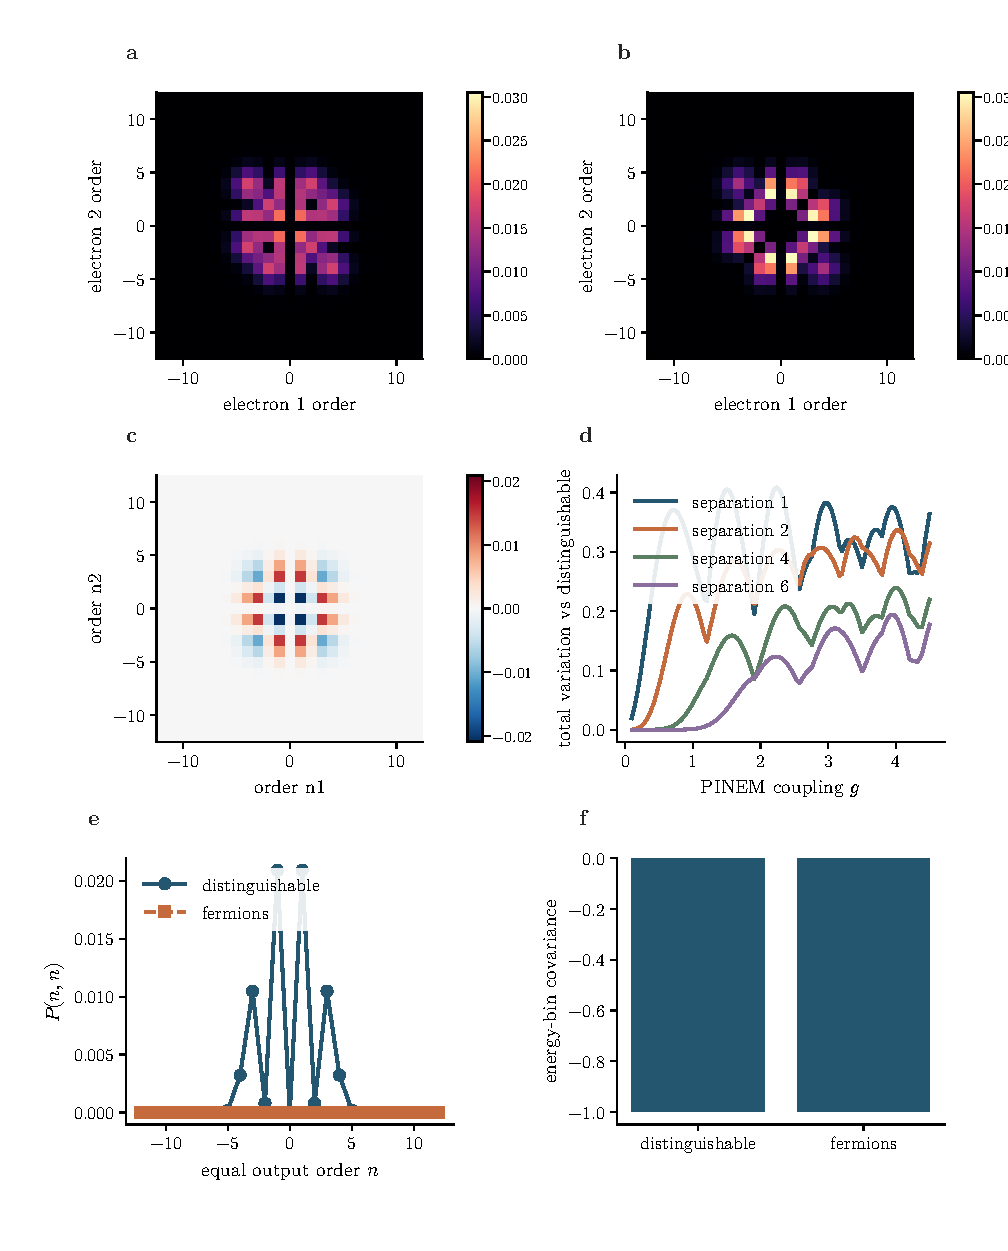
\includegraphics[width=0.96\linewidth,height=0.70\textheight,keepaspectratio]{two_electron_fermionic_interference.pdf}
\caption{\textbf{双电子能量通道中的费米交换干涉}\quad 先让两电子分别经历同一个单粒子 PINEM 幺正变换，再比较可分辨粒子与全同费米子的联合能量计数。即使两条输入能量轨道在 Hilbert 空间正交，经同一幺正调制后仍然正交，它们也可在同一输出能量\emph{测量通道}中都有非零幅度；联合概率中的两条不可分辨路径相减，因此出现交换修正，使对角附近的同时占据受到抑制。 图中把联合计数、由 Slater 行列式产生的交换项、交换可见度以及能量通道协方差并列。它只描述统计交换造成的关联，不包含额外的电子—电子相互作用势。}
\label{fig:ch06-novel-extensions--26-two-electron-fermionic-interference}
\end{figure}

数值实现中，在同一个单电子 PINEM 幺正变换 $U$ 下，比较可分辨粒子乘积态和归一化反对称态：
\[\Psi_F(n_1,n_2)=\frac{u_a(n_1)u_b(n_2)-u_b(n_1)u_a(n_2)}{\sqrt{2(1-|\langle u_a|u_b\rangle|^2)}},\quad P_F=|\Psi_F|^2,\quad P_D=\tfrac12(|u_a|^2\otimes|u_b|^2+|u_b|^2\otimes|u_a|^2).\]
$u_{a,b}$ 由初态分别作单电子演化获得，图示耦合 $g=2.0$、入射模式间隔 2、边带截断 $|n|\le12$；交换修正 $\Delta P=P_F-P_D$，交换可见度为总变差距离 $D_{\rm TV}=\tfrac12\sum|P_F-P_D|$。协方差为 $\langle n_1n_2\rangle-\langle n_1\rangle\langle n_2\rangle$。图中没有显式电子—电子势，故不能把 $\Delta P$ 归因于库仑相互作用。


先不加入库仑势，只看两个平行自旋电子。若两轨道在同一点取值相同，即令 $1=2=x$，\cref{eq:ch06-1} 的分子变成


\begin{equation*}
\phi_a(x)\phi_b(x)-\phi_b(x)\phi_a(x)=0.
\end{equation*}


因此 $|\Psi_A(x,x)|^2=0$。这就是交换孔最直接的来源：两个电子出现在同一单粒子状态的两条交换路径振幅完全相消。这里没有使用任何排斥势，所以这一零点不能解释成经典库仑排斥。

若两个轨道逐渐分离，重叠 $|S|$ 变小，交换交叉项只在两轨道同时有幅度的区域存在；若再用自旋或时间标签把两电子变得可分辨，就不再需要把两条路径相干相减。后面的交换可见度图因此把 $|S|$ 或相对延迟作为控制参数，而相互作用图则另行改变 $V$ 的强度。两类扫描的物理作用不同。

最后必须排除最容易混淆的解释：一个被探测到的关联峰究竟由输入态反对称性、相互作用动力学，还是仪器选择性造成？这三者需要在同一前向模型中分别关掉。
相对延迟、轨道重叠和自旋主要改变两电子的可分辨性；相互作用强度和作用时间主要改变动力学关联。把这两类参数放在不同坐标轴上扫描，就能判断联合计数中的抑制究竟来自交换，还是来自真实相互作用。


交换孔、HOM 型可见度、联合边带和施密特（Schmidt）数都是从同一个两体态得到的不同观测。它们分别强调局域排斥、不可分辨性、实验联合计数和非可分离程度。只有把这些量放回同一密度矩阵中比较，才不会把不同来源的“关联”混为一谈。

\begin{figure}[!htbp]
\centering
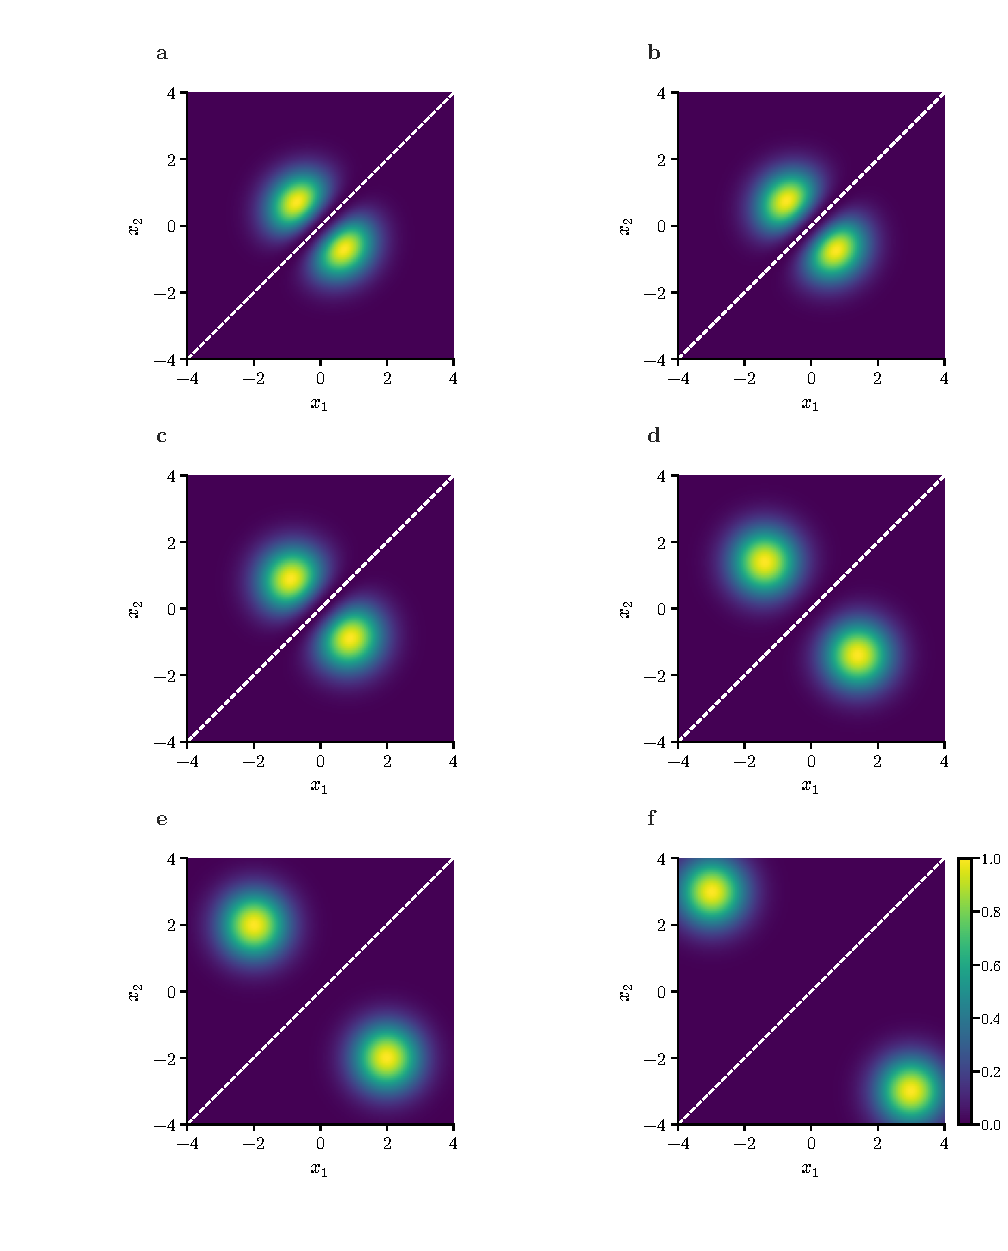
\includegraphics[width=0.96\linewidth,height=0.70\textheight,keepaspectratio]{exchange_hole.pdf}
\caption{\textbf{交换孔的空间尺度}\quad 两个高斯轨道组成的反对称双粒子态在 $r_1=r_2$ 处严格为零，因此联合位置概率出现交换孔。轨道重叠越大，交换孔的空间形状随之改变；对平行自旋的理想同位置探测，对角线始终严格为零；当两轨道几乎正交时，交换修正随之消失。}
\label{fig:ch06-story-extensions--33-exchange-hole}
\end{figure}

数值实现中，高斯轨道与两电子的规范化反对称叠加为
\[\phi_\pm(x)=\pi^{-1/4}e^{-(x\mp d/2)^2/2},\quad S=\langle\phi_+|\phi_-\rangle=e^{-d^2/4},\quad \Psi_F(x_1,x_2)=\frac{\phi_+(x_1)\phi_-(x_2)-\phi_-(x_1)\phi_+(x_2)}{\sqrt{2(1-S^2)}}.\]
六个面板分别取 $d=0.35,0.8,1.6,2.8,4,6$，以 $260^2$ 个位置点覆盖 $x_1,x_2\in[-4,4]$，绘制反对称组合的 $|\phi_+(x_1)\phi_-(x_2)-\phi_-(x_1)\phi_+(x_2)|^2$。每格再按该格的最大值归一化，而不是按联合概率的积分归一化；因此只比较交换孔的形状，不比较绝对计数。理论概率的归一化因子为 $[2(1-e^{-d^2/2})]^{-1}$；无论轨道位移如何改变，费米反对称性始终要求 $P_F(x,x)=0$。




\medskip



\begin{figure}[!htbp]
\centering
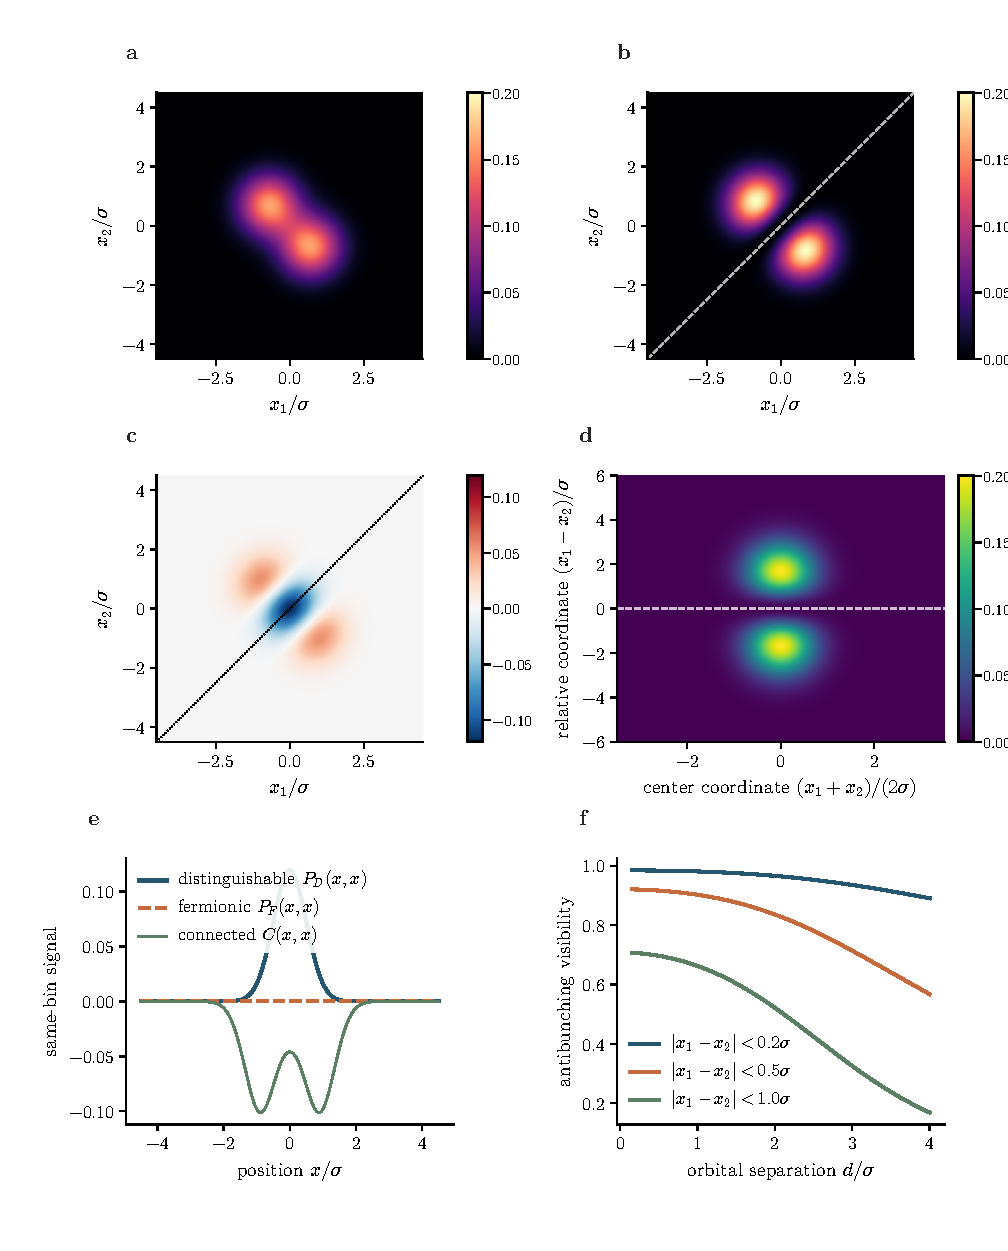
\includegraphics[width=0.96\linewidth,height=0.70\textheight,keepaspectratio]{two_particle_correlations.pdf}
\caption{\textbf{两粒子观测量的比较}\quad 这组图把“交换效应究竟长什么样”拆成多个互相呼应的读出。左上和中上给出可分辨粒子与费米子的联合密度基准，右上则直接显示交换修正 $P_F-P_D$，把反相关区域从背景中扣出来。左下改用中心坐标与相对坐标表示同一两体分布，可以一眼看到交换孔严格锁定在零相对距离处；中下的对角切片进一步展示 Pauli 抑制如何压低同位点联合计数。最右下则把这一理想交换孔与真实探测条件联系起来：随着探测窗口变宽，实验可见的反聚束可见度显著降低。全部面板仍属于 $V=0$ 的交换基准，因此它们建立的是“纯统计反对称性”应有的视觉特征，而不是把交换误读成额外动力学纠缠。}
\label{fig:ch06-story-universal--12-two-particle-correlations}
\end{figure}

六幅图完全以同一归一化反对称双高斯态计算，不再引入缺少微观动力学依据的“相互作用代理”。令
\[P_D(x_1,x_2)=\tfrac12\bigl(|\phi_+(x_1)\phi_-(x_2)|^2+|\phi_-(x_1)\phi_+(x_2)|^2\bigr),\qquad P_F=|\Psi_F|^2,\]
\[\Delta P=P_F-P_D,\quad C_F(r)=\ii nt_{|x_1-x_2|<r}\!P_F(x_1,x_2)\dd x_1\,\dd x_2,\quad C_D(r)=\ii nt_{|x_1-x_2|<r}\!P_D(x_1,x_2)\dd x_1\,\dd x_2.\]
使用轨道间隔 $d=1.40$，$x\in[-4.5,4.5]$（320 点），有限网格积分前对 $P_{D,F}$ 分别归一化；重叠扫描 $d\in[0.15,4]$（300 点），邻近窗口阈值 $r\in[0,2.5]$（95 点）。严格有 $P_F(x,x)=0$，但任何有限分辨率的邻近区计数 $C_F(r>0)$ 不必为零。

具体到各面板，(a,b) 使用位移 $d=1.40$ 的两高斯轨道，在 $[-4.5,4.5]^2$ 的 $320^2$ 位置网格上分别计算并归一化 $P_D$ 和 $P_F$。(c) 绘制 $P_F-P_D$，色限关于零对称。(d) 改变量为质心 $X=(x_1+x_2)/2$ 与相对位移 $r=x_1-x_2$，取 $240\times280$ 网格，展示 $P_F(X+r/2,X-r/2)$；Jacobian 为 1。(e) 比较 $P_D(x,x)$、$P_F(x,x)$ 及连通相关 $C(x,x)=P_F(x,x)-p_1(x)p_2(x)$。(f) 扫描轨道间距 $d\in[0.15,4]$ 共 220 点，对检测窗口 $|x_1-x_2|<r_c$、$r_c=0.2,0.5,1.0$，计算邻近区概率 $Q_{F,D}$ 并显示 $1-Q_F/Q_D$。有限检测窗口影响反聚束可见度，而 $P_F(x,x)=0$ 在任何 $d$ 下仍严格成立。


\medskip
费米交换来自总态反对称性，不需要粒子间存在相互作用；真实两体势则改变相对运动并产生额外动力学关联，因此“交换孔”和“库仑关联”不能互相替代。

联合能量边带 $P(n_1,n_2)$ 及其连通部分 $C=P-P_1P_2$ 是区分独立散射与相关散射的直接统计量，但普通 Schmidt 模式数对不可分辨费米子不能无条件解释为纠缠度量。

Kapitza--Dirac 脉冲把实空间两体关联映射到动量衍射图样，为检验相互作用和交换效应提供了清晰的基准问题。

真实自由电子实验已经能够按事件重构双电子联合态；超冷原子两体衍射只保留为受控方法学基准。判断新方案时，应优先比较联合密度矩阵、纯度和费米子适用的纠缠指标，而不是只比较一张反相关热图。


前面几个图都在无相互作用的 Slater 态上识别交换孔，因此仍缺一个关键的对照：在两束电子真正相遇时，库仑动力学会在交换基准之外增加哪些结构？这不需要先把真实三维束流的全部细节都放进数值模型。可以先使用一维相对运动的受控模型，把交换的\textbf{运动学零点}和相互作用造成的\textbf{散射相位}明确分开，再讨论它能够外推到哪些实验。

考虑沿同一有效坐标传播的两个等质量、同自旋费米子，并取 $\hbar=m=1$。两体波函数满足
\begin{equation}
\ii\partial_t\Psi(x_1,x_2,t)=\left[-\frac12(\partial_{x_1}^2+\partial_{x_2}^2)
+\frac{u}{\sqrt{(x_1-x_2)^2+a^2}}\right]\Psi(x_1,x_2,t).
\label{eq:ch06-soft-coulomb}
\end{equation}
其中 $u$ 是无量纲相互作用强度，$a>0$ 是短距离软核参数。这个势只是一维有效散射基准，\emph{不能}在未说明横向束缚及屏蔽环境时直接解释为真空中自由电子的三维库仑势。选取相向传播的归一化高斯单粒子包络
\begin{equation}
\varphi_L(x)\propto\exp[-(x+x_0)^2/(4\sigma^2)+\ii p_0x],\qquad
\varphi_R(x)\propto\exp[-(x-x_0)^2/(4\sigma^2)-\ii p_0x],
\label{eq:ch06-collision-packets}
\end{equation}
并由它们构成规范化反对称初态
\begin{equation}
\Psi_0(x_1,x_2)=\mathcal N
[\varphi_L(x_1)\varphi_R(x_2)-\varphi_R(x_1)\varphi_L(x_2)].
\label{eq:ch06-collision-initial}
\end{equation}
这里 $\mathcal N$ 是按实际离散积分计算的归一化因子，而不是将有限重叠误当成零。由于相互作用势满足 $V(x_1,x_2)=V(x_2,x_1)$，它与粒子交换算符对易，因此无论 $u$ 如何改变，同自旋费米态在任何时刻都严格保持 $\Psi(x,x,t)=0$。这说明“对角线密度是否为零”\emph{不能}单独用来测量库仑相互作用；必须比较交换孔附近的分布、相对运动和有限探测窗口中的符合概率。

引入质心坐标 $R=(x_1+x_2)/2$、相对坐标 $r=x_1-x_2$。二者的运动分解为
\begin{equation}
-\frac12(\partial_{x_1}^2+\partial_{x_2}^2)
=-\frac14\partial_R^2-\partial_r^2,
\qquad V=\frac{u}{\sqrt{r^2+a^2}}.
\label{eq:ch06-relative-hamiltonian}
\end{equation}
相对波函数因 Pauli 原理是奇函数，但软库仑势会改变不同相对动量成分的散射相移。因此自由费米和相互作用费米的\textbf{对角线均为零}，然而它们的最终相对坐标概率 $p(r,t)=\int\dd R\,|\Psi(R+r/2,R-r/2,t)|^2$ 可以不同。实际像素总有有限宽度，较稳健的观测量是
\begin{equation}
C_{r_c}(t)=\ii nt_{|x_1-x_2|<r_c}\!\dd x_1\dd x_2\,
|\Psi(x_1,x_2,t)|^2.
\label{eq:ch06-close-count}
\end{equation}
对这个量应分别求 $u=0$ 与 $u>0$ 的预测，并让两者通过相同的探测器响应，才能把动力学抑制与纯交换孔分开。

\begin{figure}[!htbp]
\centering
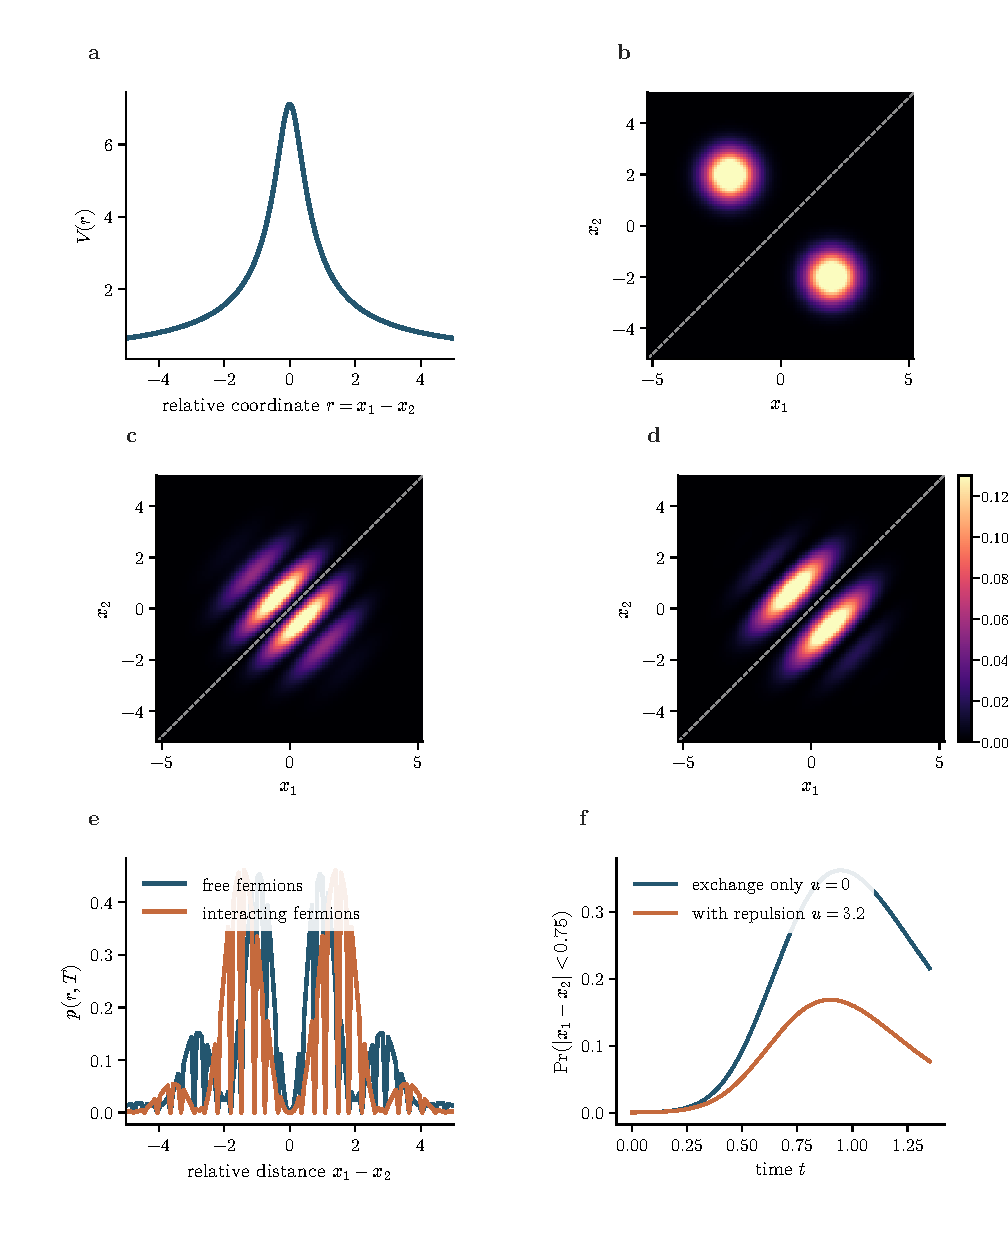
\includegraphics[width=0.97\linewidth,height=0.70\textheight,keepaspectratio]{two_electron_collision.pdf}
\caption{\textbf{带相互作用的双电子迎面散射与交换基准}\quad (a) 一维软核相对势；(b) 初始反对称两高斯波包的联合密度；(c) 在同一初态下取 $u=0$ 的自由散射终态；(d) 打开 $u=3.2$ 后的终态，两者仍保留 Pauli 对角零点，但离对角线的密度重排不同；(e) 将终态投影到相对坐标，直接看散射相位如何改变分离概率；(f) 随时间积分有限邻近窗口中的符合概率，从交换基准上辨识附加的相互作用效应。六面板全部由同一二维时变 Schrödinger 方程数值演化，未把经验退相干或所谓“纠缠百分比”偷偷乘进结果。}
\label{fig:ch06-two-electron-collision}
\end{figure}

图中统一采用\cref{eq:ch06-soft-coulomb,eq:ch06-collision-packets}，且 $\hbar=m=1$、高斯位置中心为 $x_0=2.0$、宽度 $\sigma=0.65$、相向中心动量 $p_0=1.8$。空间周期计算盒为 $[-9,9)$，取 $N_x=176$ 点，积分权重为 $(\Delta x)^2$；初态反对称化以后再次规范化为总概率 1。(a) 绘 $V(r)=u/\sqrt{r^2+a^2}$，参数为 $u=3.2,a=0.45$，显示 $r\in[-8,8]$ 中央区。(b) 为 $t=0$ 的初态联合人口 $|\Psi_0|^2$。(c,d) 均演化到 $T=1.35$，分别取 $u=0$ 与 $u=3.2$；使用二阶 Strang 分裂的 180 个时间步，单步为
\[
\Psi(t+\Delta t)\simeq \ee^{-\ii V\Delta t/2}\mathcal F^{-1}
\!\left[\ee^{-\ii(k_1^2+k_2^2)\Delta t/2}\,\mathcal F
[\ee^{-\ii V\Delta t/2}\Psi(t)]\right],\qquad
\Delta t=1.35/180.
\]
这里 $V$ 在自由基准中置零，傅里叶波数由周期 FFT 的实际频率确定，并未额外加入吸收边界。(e) 对同一终态的 $P(x_1,x_2)$ 依照 $r=x_1-x_2$ 在 $[-8,8]$ 的 200 个等宽箱中累积，箱总量除以箱宽而成为相对坐标概率密度。(f) 每一时间步计算 $C_{r_c}$，采用 $r_c=0.75$ 的严格不等式，并绘出自由交换基准与相互作用结果。不同面板的空间概率均按同一网格积分解释；短距离参数 $a$ 是可见的现象学调节量，不对应特定实验中的固定库仑长度。该时间传播保持总范数与交换反对称性，具体复现检查见 Python 脚本及根目录数值测试。


图中最后一格还有一个实验设计上的意义。若只画严格同位点 $P(x,x)$，两个模型永远都是零，无法区分任何动力学；把可测的邻近窗口 $r_c$ 和事件到达时间放进统计量后，才出现真正对相互作用敏感的量。对真实自由电子束，这一步还不够：需要恢复三维相对运动、纵向--横向纠缠、相对论修正和探测器符合窗口，但受控的一维计算已经说明接下来应该测什么、哪些信号没有判别力。


交换反对称性的空间零点与两体纠缠并不是同一个判据。为了让测量资源问题有可复核的数量级，可以用两比特截断中的一个物理密度矩阵作示例，而不把它冒充真实自由电子实验的完整状态。考虑按 $|00\rangle,|01\rangle,|10\rangle,|11\rangle$ 排序的
\begin{equation}
\rho=\begin{pmatrix}
q/2&0&0&0\\
0&(1-q)/2&c&0\\
0&c^*&(1-q)/2&0\\
0&0&0&q/2
\end{pmatrix},\qquad |c|\le\frac{1-q}{2}.
\label{eq:twoelectron-example-density}
\end{equation}
其部分转置的四个本征值分别为 $(1-q)/2,(1-q)/2,q/2+|c|,q/2-|c|$。将负本征值的绝对值求和，得到负性
\begin{equation}
\mathcal N(\rho)=\max\!\left(0,|c|-\frac q2\right).
\label{eq:twoelectron-example-negativity}
\end{equation}
例如 $q=0.10$、$|c|=0.12$ 对应 $\mathcal N=0.07$；这只是无量纲量，不是“有百分之七的电子已经纠缠”。要实验辨认如此小的非对角相干项，既要在能量基估计 $q$，也要使用相位敏感测量估计 $C=2\operatorname{Re}c$。

若总共有 $N$ 个独立的有效电子对，将其中比例 $f$ 分给相干测量，其余分给人口测量，并假设相位基具有已标定可见度 $V$，利用二项分布的方差传播可得
\begin{equation}
\operatorname{Var}(\widehat{\mathcal N})\simeq\frac{A}{fN}+\frac{B}{(1-f)N},\qquad
A=\frac{1-(VC)^2}{4V^2},\quad B=\frac{q(1-q)}4.
\label{eq:twoelectron-dose-variance}
\end{equation}
在 $|c|>q/2$ 且相位已对准使 $c$ 可取实时，这个估计式才对应非零负性的局域线性误差。对 $f$ 求导，令 $-A/f^2+B/(1-f)^2=0$，得到
\begin{equation}
f_*=\frac{\sqrt A}{\sqrt A+\sqrt B}.
\label{eq:twoelectron-dose-optimum}
\end{equation}
这说明测量设置不能机械地平均分配计数：对某一参数最敏感的读出可能最费剂量。然而 $N$ 增长只能压低统计噪声；若 $V$ 的标定误差不随 $N$ 下降，由 $c\propto C_{\rm obs}/V$ 产生的系统误差最终会形成下限。要证明弱纠缠，必须同时报告相位基标定和完整探测响应，而不仅是更深的相关性热图。

联合概率已经给出了可观测的相关结构。要从有限计数中可靠地辨认这些结构并反推出模型参数，还需要把探测器响应和统计推断一起纳入前向模型。

\clearpage
\par\medskip 对任意相同的单电子幺正变换 $U\otimes U$，两条初始正交轨道的整体内积保持为零；不过它们在某一固定探测像素或能量通道的局部幅度可以重叠，因此观测到的交换干涉仍然非零。区分这两个“重叠”能够避免把局域交换孔误写成输入态间的非正交性，更不能把无相互作用的 Slater 行列式直接解释为库仑产生的多体纠缠。


\noindent \figref{fig:ch06-novel-extensions--26-two-electron-fermionic-interference}：六面板计算逐项核对。\par\noindent (a,b) 先计算 $u_a(n)=U_{n,a}$、$u_b(n)=U_{n,b}$（输入阶相隔 2），分别求对称平均的可分辨联合概率 $P_D$ 和反对称 $P_F$；(c) $\Delta P=P_F-P_D$；(d) 扫 $g\in[0.1,4.5]$、输入阶间隔 $1,2,4,6$，取 $D_{\rm TV}=\tfrac12\sum_{ij}|P_F-P_D|$；(e) 取矩阵对角元 $P_F(n,n)$ 与 $P_D(n,n)$，前者严格为 0（计算舍入除外）；(f) 用 $\langle n_1n_2\rangle-\langle n_1\rangle\langle n_2\rangle$ 对比两种计数。单电子核 $U_{nk}=i^{n-k}J_{n-k}(2g)$ 使用有限能量截断 $|n|\le12$（扫耦合时 $|n|\le14$）；每个有限矩阵生成的双电子概率在显示前重新归一。\emph{没有}添加相互作用势。


\par\bigskip
\noindent{\small\textit{参考文献}\par\vspace{2pt}
\begin{enumerate}
\item \phantomsection\label{ch05-ref1}Wu, D.; Li, J.; Jiang, Y.; Liu, Y. Coherent Control of Three-Level System Using Shaped Free Electrons. \emph{Physical Review Letters} 137, 063601 (2026). \href{https://doi.org/10.1103/l2y4-tpzb}{\nolinkurl{doi:10.1103/l2y4-tpzb}}.
\item \phantomsection\label{ch05-ref2}Gorini, V.; Kossakowski, A.; Sudarshan, E. C. G. Completely positive dynamical semigroups of N-level systems. \emph{Journal of Mathematical Physics} 17, 821--825 (1976).
\item \phantomsection\label{ch05-ref3}Lindblad, G. On the generators of quantum dynamical semigroups. \emph{Communications in Mathematical Physics} 48, 119--130 (1976).
\item \phantomsection\label{ch05-ref4}Velasco, C. I.; Di Giulio, V.; García de Abajo, F. J. Free-electron decoherence: Theory and applications. \emph{Physical Review B} 113, 235433 (2026). \href{https://doi.org/10.1103/f35f-l1l1}{\nolinkurl{doi:10.1103/f35f-l1l1}}.
\item \phantomsection\label{ch06-ref1}Becker, A.; Koutentakis, G. M.; Schmelcher, P. Two-body Kapitza--Dirac scattering of one-dimensional ultracold atoms. \emph{Physical Review Research} 8, 013297 (2026). \href{https://doi.org/10.1103/rdsn-stlq}{\nolinkurl{doi:10.1103/rdsn-stlq}}. 该文研究接触相互作用超冷原子，本书仅将其作为两体衍射的受控基准。
\item \phantomsection\label{ch06-ref2}Haindl, R. et al. Coulomb-correlated electron number states in a transmission electron microscope beam. \emph{Nature Physics} 19, 1410--1417 (2023). \href{https://doi.org/10.1038/s41567-023-02067-7}{\nolinkurl{doi:10.1038/s41567-023-02067-7}}.
\item \phantomsection\label{ch06-ref3}Tziperman, O. et al. Two-electron quantum walks for probing entanglement and decoherence in an electron microscope. \emph{Nature Physics} 22, 763--769 (2026). \href{https://doi.org/10.1038/s41567-026-03254-y}{\nolinkurl{doi:10.1038/s41567-026-03254-y}}.
\end{enumerate}
}
